\section{1. Genes, Proteins, Databases, Genome annotation}

\begin{framed}
\textbf{Learning outcomes}\\
\begin{itemize}
\item 1
\item 2
\item 3
\end{itemize}
\end{framed}

\subsubsection{Biological background}

A large part of bioinformatics deals with the analysis of biological sequences.
These sequences originate from organic macromolecules that play important roles in cells.
In the first section of this chapter, we describe these macromolecules, their sequences, and the biological processes involved in generating their active structures and maintaining these.

As such, this section provides important background material for the entire course.
Depending on your background, parts of this section might seem redundant, in which case this section can function as a refresher.
Later chapters assume you are familiar with this section.


\bigskip
\centerline{\rule{13cm}{0.4pt}}
\bigskip

\paragraph{Nucleic acids}

Deoxyribonucleic acid (\gls{term-dna}) carries the genetic information of organisms. Ribonucleic acid (\gls{term-rna}) is involved in the protein expression and is also the genetic material of some viruses.
Thus, these molecules are highly important as the basis of life on Earth.
The \textbf{genome} denotes the cell's entire genetic content and \textbf{genomics} is the study of genomes.

DNA and RNA are comprised of monomers called \textbf{nucleotides}, which are comprised of three components (Figure~\ref{nucleotide}):

\begin{itemize}
\item A \textbf{pentose} sugar, where carbon residues are numbered 1' to 5' (read 1' as ``one prime'').
The type of pentose distinguishes RNA and DNA: the sugar is deoxyribose in DNA and ribose in RNA.
They are similar in structure, but deoxyribose has an H instead of an OH at the 2′ position.
\item A \textbf{phosphate} group that is attached to the 5' position of the sugar.
\item A \textbf{base} that is attached to the 1' position of the sugar.
\end{itemize}

\begin{figure}[!htbp]
\centering
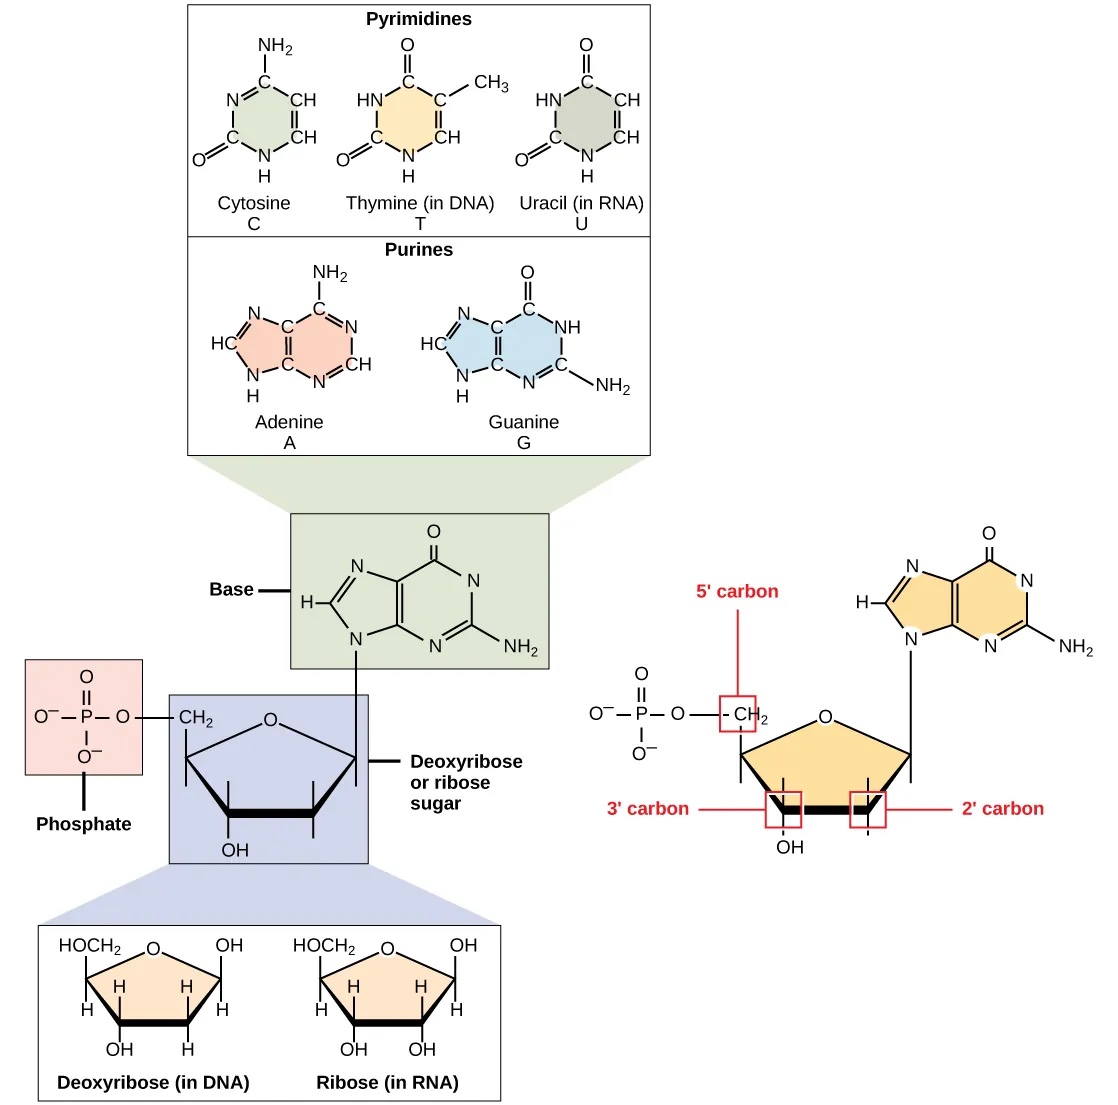
\includegraphics[width=0.9\linewidth]{files/nucleotide-1c35cedc9ecc9b60b760ac4c6644688f.jpg}
\caption[]{The components of a nucleotide.
Credits: \href{https://creativecommons.org/licenses/by/4.0}{CC BY 4.0} \cite{nucleotide_2018}.}
\label{nucleotide}
\end{figure}

The bases can be divided into two categories: purines (with a double ring structure) and pyrimidines (with a single ring structure) (Figure~\ref{nucleotide}).
DNA contains A, T, C, and G; whereas RNA contains A, U, C, and G.

\begin{framed}
\textbf{Important}\\
Nucleotides are central molecules in all life.
You do not need to remember the exact chemical structure, but you need to know the difference between DNA and RNA, the different bases and their category (purines or pyrimidines).
\end{framed}


\bigskip
\centerline{\rule{13cm}{0.4pt}}
\bigskip

\paragraph{The DNA double helix}

The DNA molecule is a polymer of deoxyribonucleotides and forms a right-handed double helix.
The sugar and phosphate are on the outside forming the helix's backbone and the bases are stacked in the interior and bind each other by hydrogen bonds.
Thereby A pairs with T via two hydrogen bonds and C pairs with G via three hydrogen bonds, they are \textbf{complementary} bases.
These pairings are also called Watson-Crick base-pairing, named after the discoverers of DNA.

% :::{figure} images/chapter1/dna.jpg
% :alt: DNA structure
% :width: 70%
% :name: dna
% 
% The DNA structure.
% Credits: {cite}`dna_2008`.
% :::
% #% Unable to use figure dna due to copyright.

\begin{figure}[!htbp]
\centering
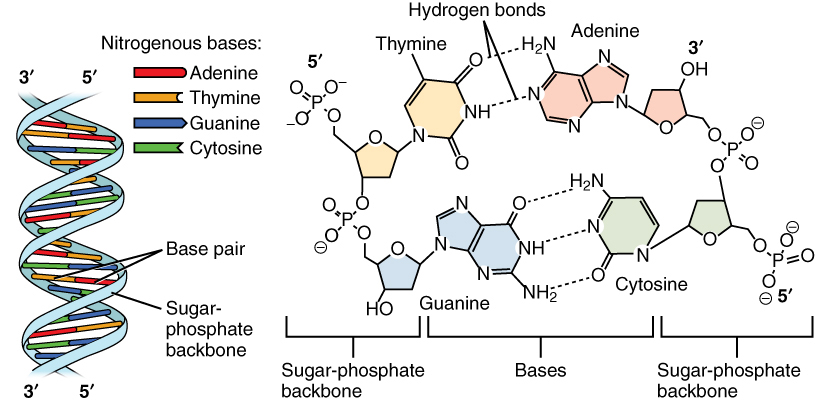
\includegraphics[width=0.8\linewidth]{files/dna_alt-0d35e3218bc7b4f7a3ade1e1f483b3ac.jpg}
\caption[]{The DNA structure.
Credits: \href{https://creativecommons.org/licenses/by/3.0/}{CC BY 3.0} \cite{dna_alt_2013}.}
\label{dna_alt}
\end{figure}

The two strands of the helix run in opposite directions, also called anti-parallel, i.e., one goes from 5' to 3' and the other from 3' to 5' (Figure~\ref{dna_alt}).
The nucleotide sequence is typically written in 5' to 3' direction.
Due to the complementarity, the base sequence of a strand can be deduced from the base sequence from the other strand.
This is called the \textbf{reverse complement}.
For example, the reverse complement of AAGT is ACTT, where both strands are given in 5' to 3' direction.


\bigskip
\centerline{\rule{13cm}{0.4pt}}
\bigskip

\paragraph{DNA replication}\label{chapter1_replication}

As the two DNA strands are only connected via hydrogen bonds, they can be separated relatively easily, for example during DNA replication (Figure~\ref{replication_alt}).
The separated strands each serve as a template on which a new complementary strand is synthesized by the enzyme DNA polymerase in 5' to 3' direction.
This mode of replication is called semiconservative.

% :::{figure} images/chapter1/replication.jpg
% :alt: Replication
% :width: 50%
% :name: replication
% 
% A) The process of DNA replication.
% Credits: [CC0 1.0](https://creativecommons.org/publicdomain/zero/1.0/) {cite}`replication_a_2013`.
% B) Semiconservative DNA replication, where the two copies each contain one original strand and one new strand.
% Credits: [CC BY-SA 2.5](https://creativecommons.org/licenses/by-sa/2.5/) {cite}`replication_b_2005`.
% :::
% #% Unable to use figure replication due to copyright.

\begin{figure}[!htbp]
\centering
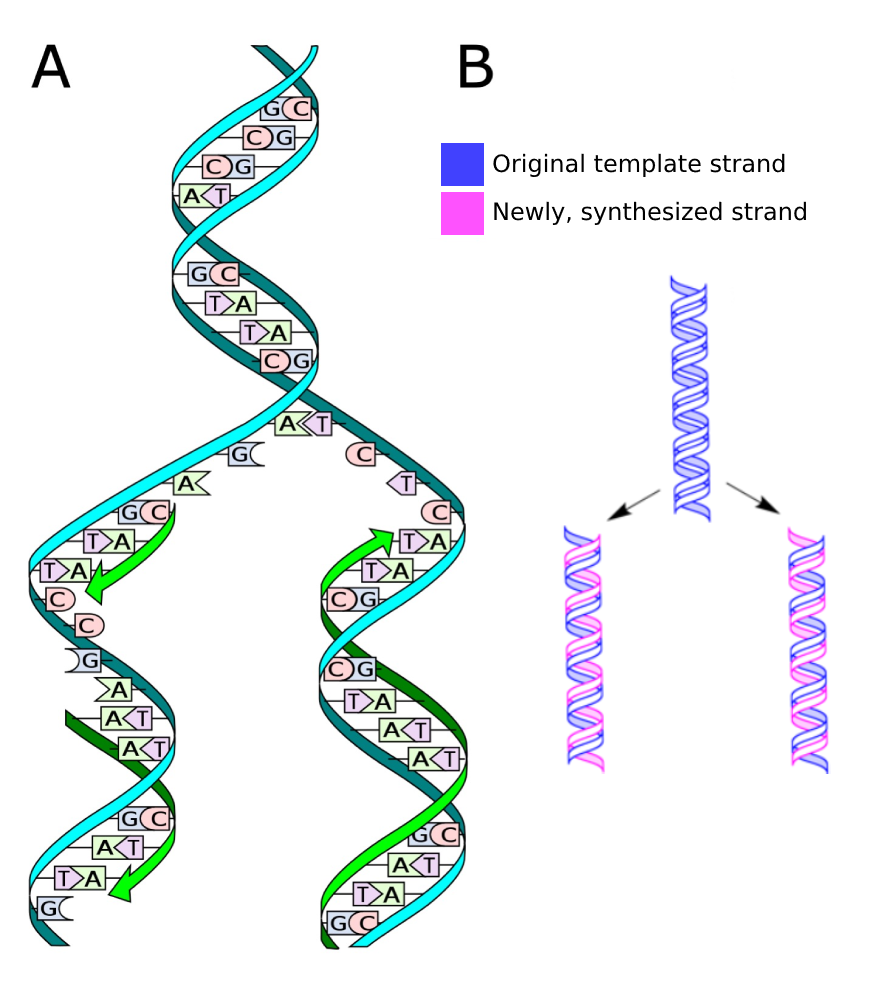
\includegraphics[width=0.5\linewidth]{files/replication_alt-f04199f765869f1200a2c0d77cd5136c.png}
\caption[]{A) The process of DNA replication.
Credits: \href{https://creativecommons.org/publicdomain/zero/1.0/}{CC0 1.0} \cite{replication_a_2013}.
B) Semiconservative DNA replication, where the two copies each contain one original strand and one new strand.
Credits: \href{https://creativecommons.org/publicdomain/zero/1.0/}{CC0 1.0} modified from \cite{replication_b_alt_2009}.}
\label{replication_alt}
\end{figure}

The error rate of DNA replication is remarkably low, about one erroneous base in 10\textsuperscript{9} bases.
This property preserves the genetic information during cell division, and also over generations.
It also leads to mutations over evolutionary time (Figure~\ref{dna_mutation}), as we will see later (Substitutions).

\begin{figure}[!htbp]
\centering
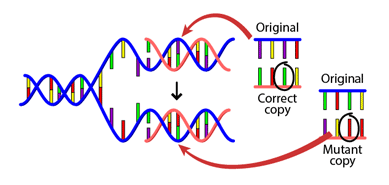
\includegraphics[width=0.5\linewidth]{files/dna_mutation-68a911a7c532b62f50f2909c59238895.png}
\caption[]{A DNA mutation that occurs during replication.
Credits: \href{https://creativecommons.org/licenses/by-nc-sa/4.0/}{BY-NC-SA 4.0} \cite{dna_mutation_2020}.}
\label{dna_mutation}
\end{figure}


\bigskip
\centerline{\rule{13cm}{0.4pt}}
\bigskip

\paragraph{RNA, transcription, and splicing}\label{chapter1_rna_transcription_splicing}

During transcription, RNA polymerase reads the template strand (also called noncoding strand) in the 3' to 5' direction (Figure~\ref{transcription}).
This produces an RNA molecule from 5' to 3', which is a copy of the coding strand.
During transcription thymine is replaced by uracil.
In contrast to DNA, RNA does not form a stable double helix.
RNA is mainly single stranded, but most RNAs show intramolecular base pairing between complementary bases.

There are four major types of RNA:

\begin{itemize}
\item Messenger RNA (mRNA): RNA molecules that will later be translated into proteins and therefore serve as a `messenger' in protein production.
\item Ribosomal RNA (rRNA): the primary component of ribosomes (the `powerplants' of a cell).
\item Transfer RNA (tRNA): functions as `adapter molecule' that serve as the physical link between mRNA and the amino acid sequence of a protein during translation.
\item MicroRNA (miRNA): non-coding RNA molecules of 21-23 nucleotides involved in RNA silencing and post-transcriptional regulation of gene expression.
\end{itemize}

\begin{figure}[!htbp]
\centering
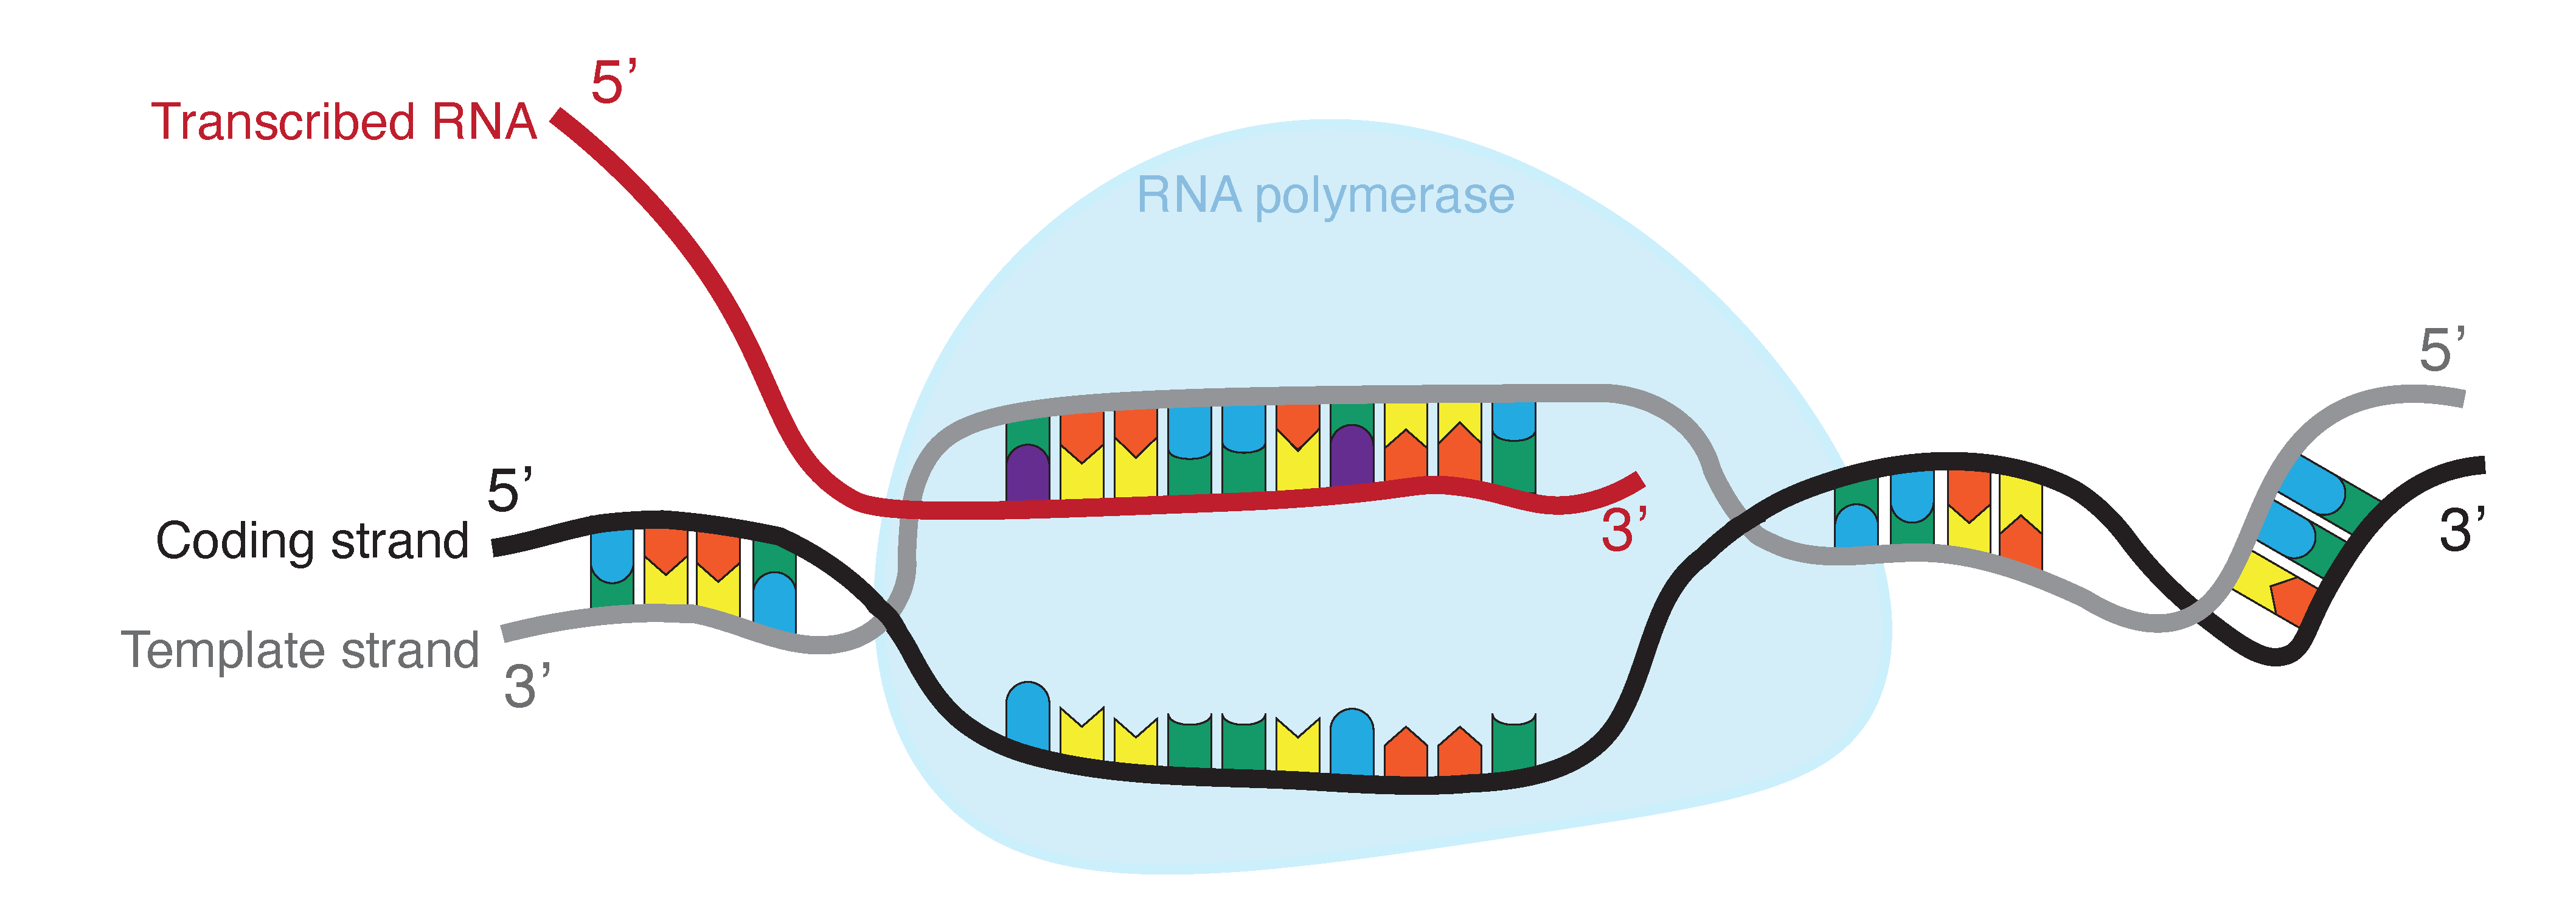
\includegraphics[width=0.7\linewidth]{files/transcription-a75e6e7573d01b067818d6dc4aa4f2fa.png}
\caption[]{RNA is produced by transcribing DNA: as such, it is a direct copy of the information contained in the DNA.
Where DNA contains thymine (T, indicated in blue), RNA contains uracil (U, indicated in purple).
Credits: \href{https://creativecommons.org/licenses/by-nc/4.0/}{CC BY-NC 4.0} \cite{own_1_2024}.}
\label{transcription}
\end{figure}

In eukaryotes, precursor mRNA molecules undergo splicing.
During RNA splicing, the spliceosome protein complex removes introns: specific non-coding parts of an mRNA molecule that are not used during translation (Figure~\ref{splicing}), to create mature mRNA.
Most introns are characterized by a GU and AG dinucleotide motif in the 5' and 3' end respectively.

\begin{figure}[!htbp]
\centering
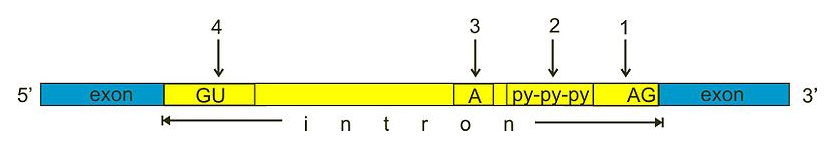
\includegraphics[width=0.7\linewidth]{files/splicing-ae129e41abb4fdbb769ee710d9e66b60.jpg}
\caption[]{During splicing, introns are removed from precursor mRNA moleculus to create mature mRNA.
Most introns contain several canonical elements that help in recognition by the spliceosome and in creating a specific secondary structure of the intronic RNA that facilitates removal: \textbf{(1)} 3' splice site, \textbf{(2)} poly pyrimidine tract, \textbf{(3)} branch site, \textbf{(4)} 5' splice site'.
Credits: \href{https://creativecommons.org/publicdomain/zero/1.0/}{CC0 1.0} \cite{splicing_2011}.}
\label{splicing}
\end{figure}


\bigskip
\centerline{\rule{13cm}{0.4pt}}
\bigskip

\paragraph{Translation}\label{chapter1_translation}

During protein translation, ribosomes synthesize polypeptides from messenger RNA (mRNA) (Figure~\ref{translation_alt}).
During this process tRNAs decode the information on the RNA into amino acids, where a codon consisting of three nucleotides encodes the information for one amino acid.

% :::{figure} images/chapter1/translation.jpg
% :alt: Translation
% :width: 70%
% :name: translation
% 
% The translation process, where ribosomes with tRNA molecules "read" codons on the mRNA using anticodons, which then get translated into their corresponding amino acids.
% These amino acids are linked together by peptide bonds to form a polypeptide chain.
% :::
% #% Unable to use figure translation due to copyright.

\begin{figure}[!htbp]
\centering
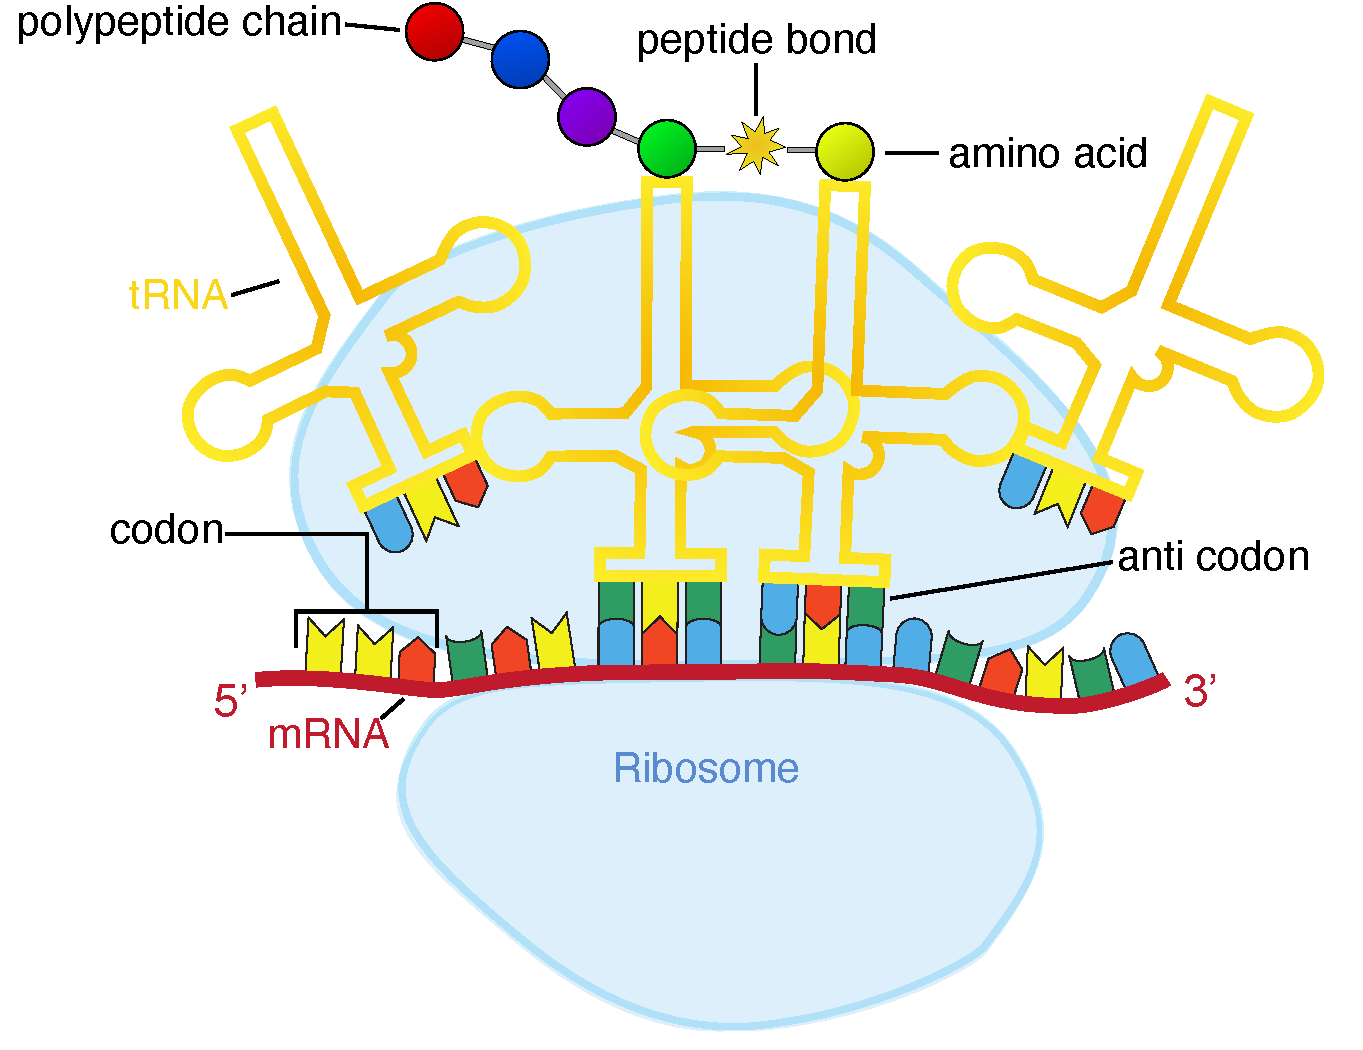
\includegraphics[width=0.7\linewidth]{files/translation_alt-47ee1f3f0d058509ab6b6043187d4a5e.pdf}
\caption[]{The translation process, where ribosomes with tRNA molecules ``read'' codons on the mRNA using anticodons, which then get translated into their corresponding amino acids.
These amino acids are linked together by peptide bonds to form a polypeptide chain.
Credits: \href{https://creativecommons.org/licenses/by-nc/4.0/}{CC BY-NC 4.0} \cite{own_1_2024}.}
\label{translation_alt}
\end{figure}

\begin{framed}
\textbf{See Also}\\
The details of transcription and translation differ between prokaryotes and eukaryotes. You can look up Chapters 15 and 16 of \href{https://openstax.org/details/books/biology-2e}{Biology 2e} to learn more.
\end{framed}

\paragraph{The genetic code}\label{chapter1_genetic_code}

The genetic code shows the correspondence between codons and amino acids (Figure~\ref{geneticcode}).
Since 64 possible codons code for 20 different amino acids, the genetic code is degenerate, i.e., most amino acids are specified by more than one codon.
Thus, the codons encoding one particular amino acid may differ in one or two of their positions.
You can notice in Figure~\ref{geneticcode} that the third codon position often differs between codons for the same amino acid.
As a result of the code degeneracy, the protein sequence can be deduced from the DNA or RNA sequence but not vice versa.

There are three codons that do not encode for an amino acid, but instead signal the end of the protein sequence, called \textbf{stop codons}.
Furthermore, translation generally starts with the start codon AUG encoding methionine.
More information of how protein information is encoded in genomes can be found in the section on genome~annotation.

\begin{figure}[!htbp]
\centering
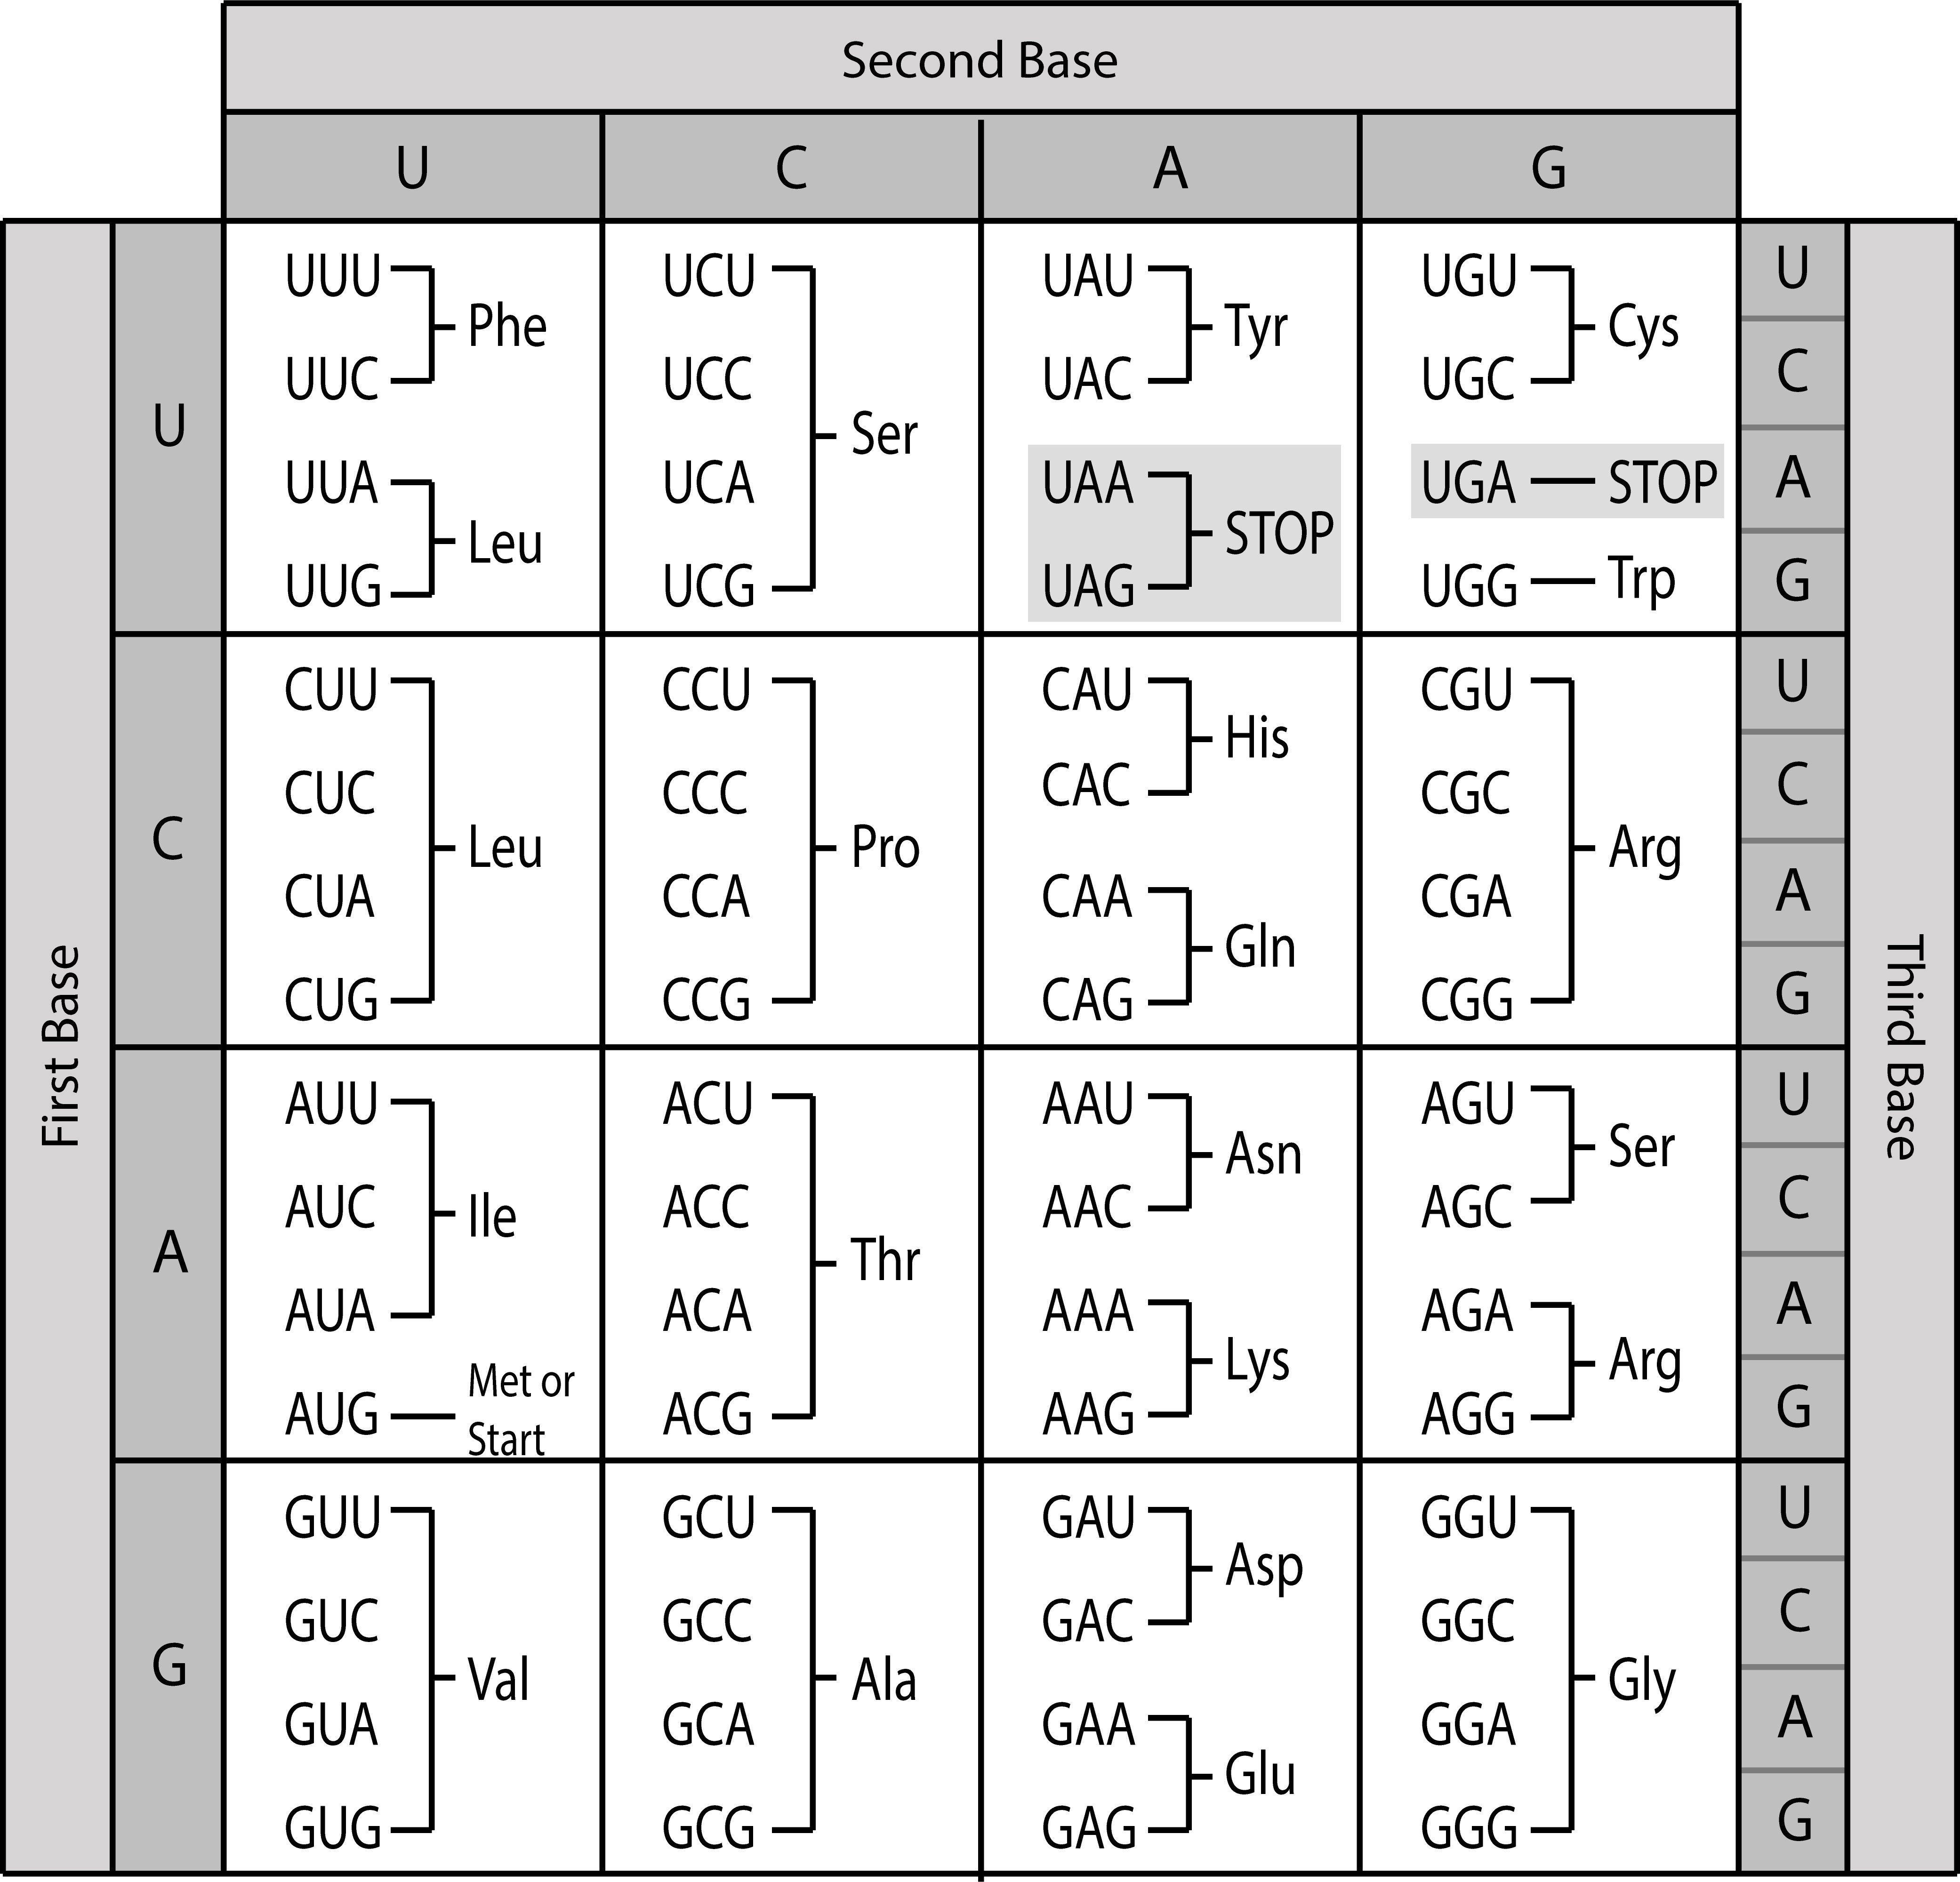
\includegraphics[width=0.8\linewidth]{files/geneticcode-3167edd785c0ef0c20cd7c489c096264.jpg}
\caption[]{The universal genetic code. Note that exceptions to this code exist, for example the vertebrate mitochondrial code.
Credits: \href{https://creativecommons.org/licenses/by/4.0}{CC BY 4.0} \cite{geneticcode_2018}.}
\label{geneticcode}
\end{figure}

\begin{framed}
\textbf{Important}\\
The universal genetic code is very important to understand how information flows from genes to proteins.
Nevertheless, you do not need to recall it, but can always look it up.
When needed, it will also be provided in the exam.
\end{framed}

\paragraph{The central dogma of molecular biology}

According to the central dogma of molecular biology, the flow of genetic information is essentially in one direction: from DNA via RNA to proteins (Figure~\ref{dogma_alt}).
Nevertheless, there are also genes that do not code for proteins, but where functional RNA is the end product. Furthermore, mobile genetic elements and viruses can encode reverse transcriptases (which can synthesize DNA from an RNA template) or RNA dependent RNA polymerases (which can replicate RNA).

% :::{figure} images/chapter1/dogma.jpg
% :alt: Central dogma
% :width: 35%
% :name: dogma
% 
% The central dogma of molecular biology.
% Credits: [CC BY-SA 3.0](https://creativecommons.org/licenses/by-sa/3.0/) {cite}`dogma_2008`.
% :::
% #% Unable to use figure dogma due to copyright.

\begin{figure}[!htbp]
\centering
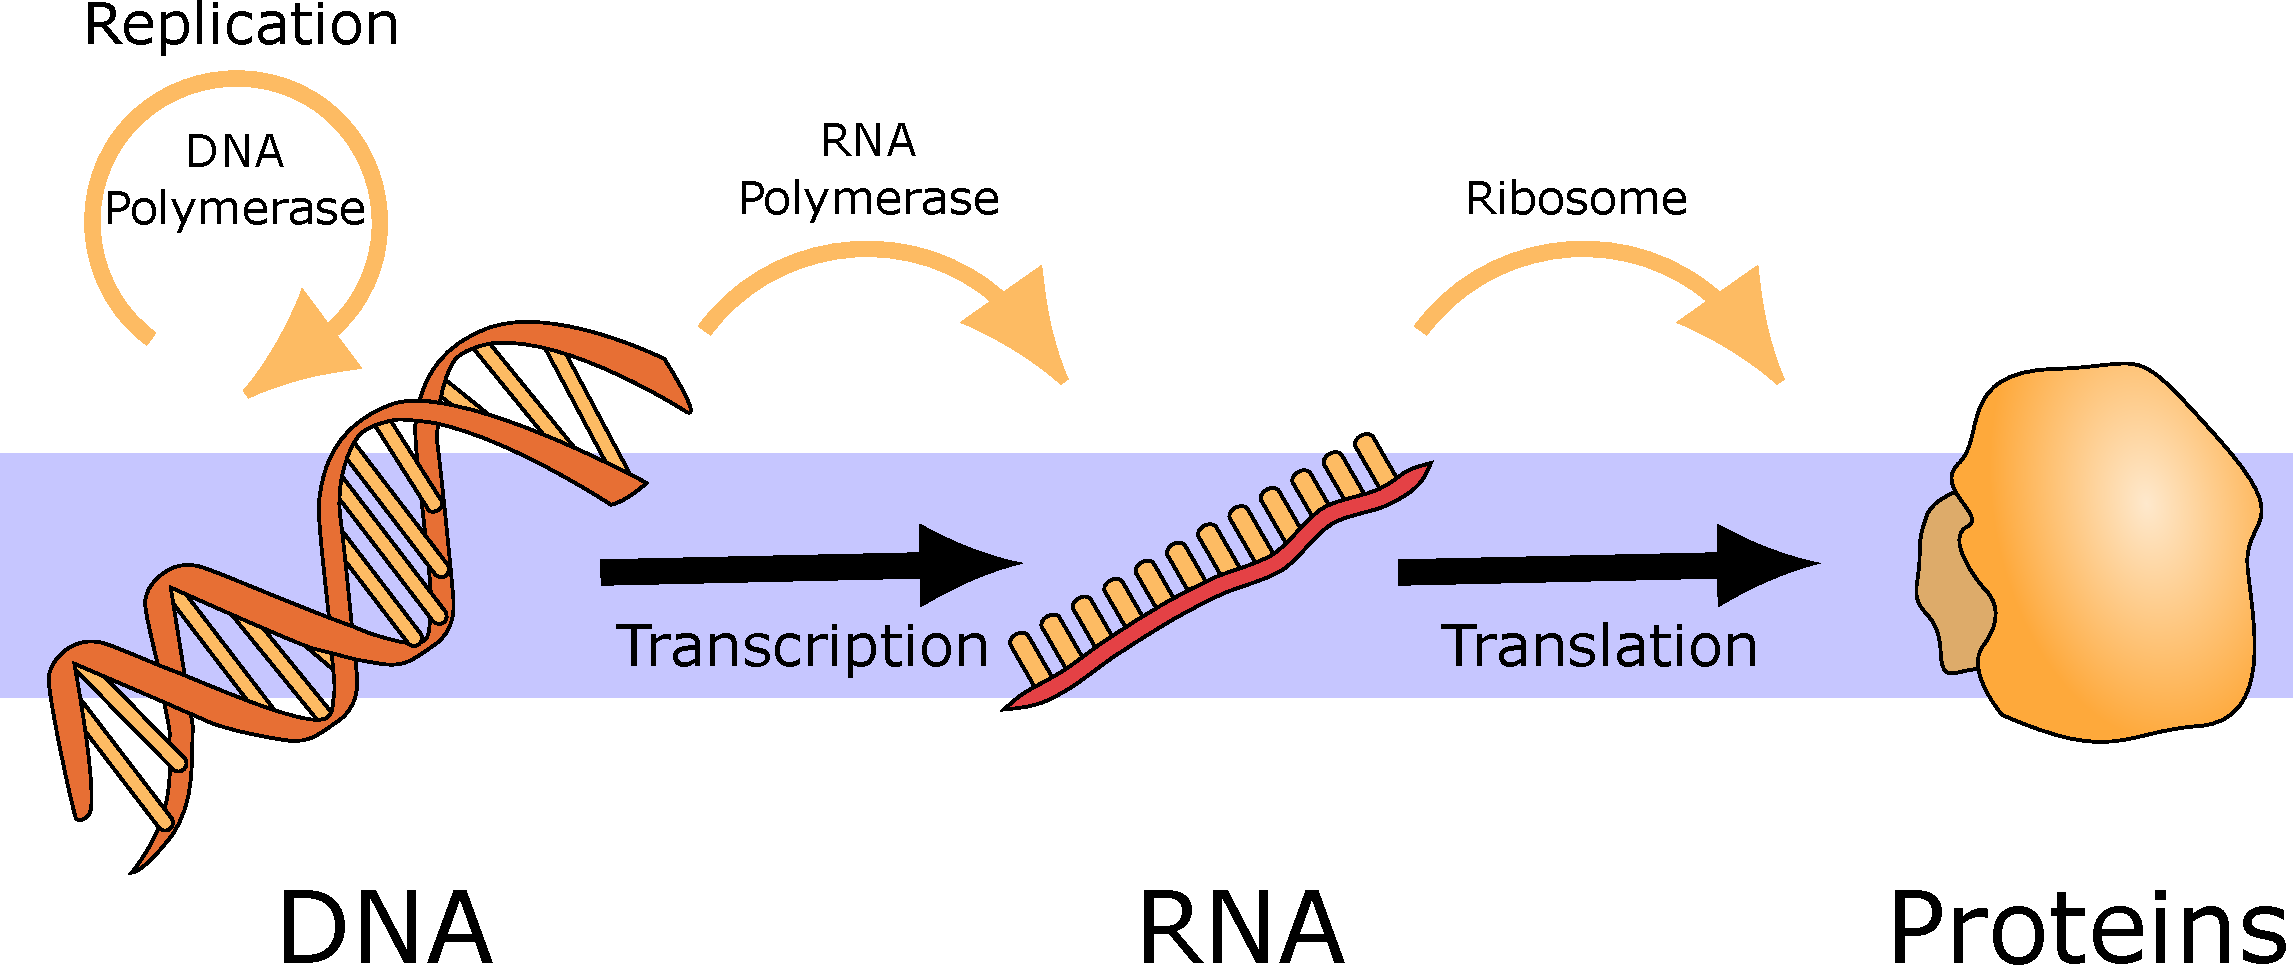
\includegraphics[width=0.8\linewidth]{files/dogma_alt-2d2dc9071cc69db13eb71dff5220b6b2.pdf}
\caption[]{The central dogma of molecular biology.
Credits: \href{https://creativecommons.org/publicdomain/zero/1.0/}{CC0 1.0} modified from \cite{dogma_alt_2008}.}
\label{dogma_alt}
\end{figure}

\paragraph{Proteins}

Proteins are large, complex macromolecules that play many important roles in the body.
They are critical to most of the work done by cells and are required for the structure, function and regulation of the body's tissues and organs.
The basic building blocks of proteins are amino acids.


\bigskip
\centerline{\rule{13cm}{0.4pt}}
\bigskip

\subparagraph{Amino acids}\label{chapter1_aminoacids}

An amino acid contains a central carbon atom (called $\alpha$-carbon, or C\textsubscript{$\alpha$}) (Figure~\ref{aminoacid}).
The $\alpha$-carbon is bound to an amino group (NH\textsubscript{2}), a carboxyl group (COOH), and a hydrogen atom. In addition, each amino acid has a specific residue (R) group.

\begin{figure}[!htbp]
\centering
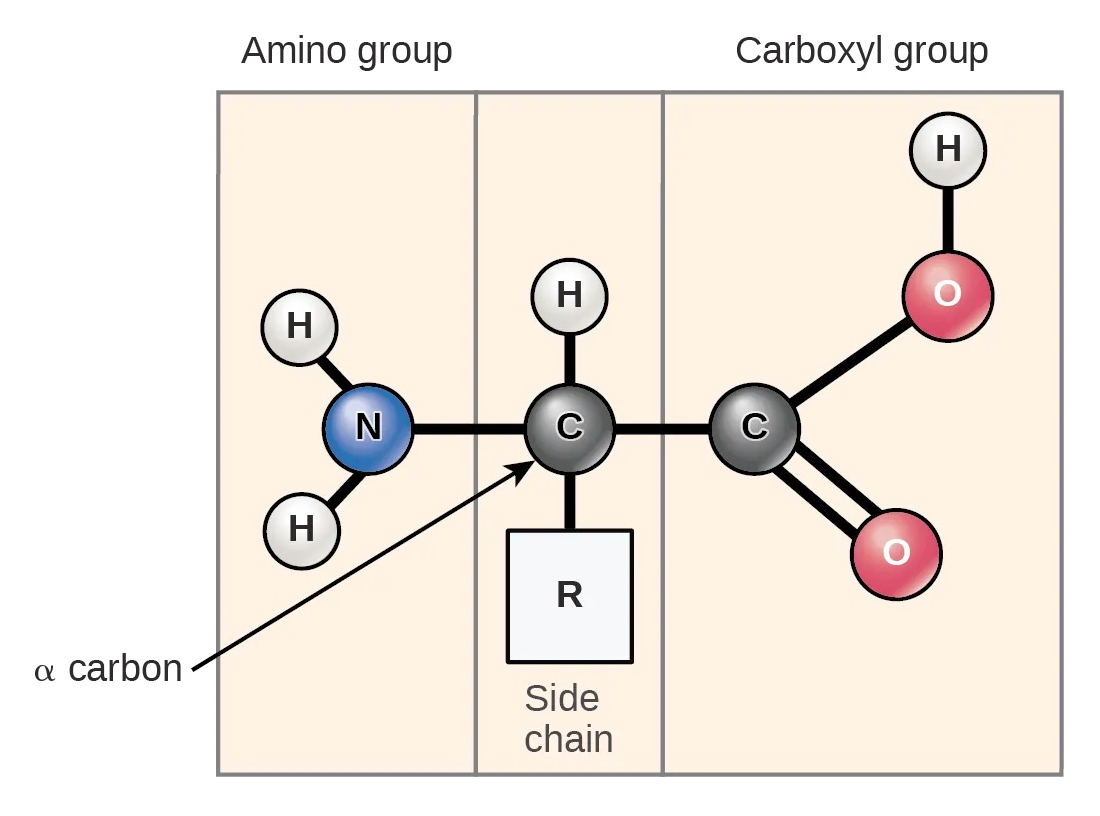
\includegraphics[width=0.6\linewidth]{files/aminoacid-43fb3a83f9ded9cb29064fb29d80b29c.jpg}
\caption[]{The structure of an amino acid.
Four elements are connected to the $\alpha$-carbon: an amino group, a hydrogen atom, a carboxyl group, and a side chain (R group).
Credits: \href{https://creativecommons.org/licenses/by/4.0}{CC BY 4.0} \cite{proteins_2018}.}
\label{aminoacid}
\end{figure}

\begin{framed}
\textbf{Important}\\
Amino acids differ in their chemical properties, which are determined by their R groups.
It is important to know (by heart) the amino acids, their one-letter and three-letter abbreviation, and their fundamental properties as given in the table.
\end{framed}

\begin{table}
\centering
\caption[]{Amino acids and their abbreviations and basic properties}
\label{aminoacidtable}
\begin{tabular}{p{\dimexpr 0.250\linewidth-2\tabcolsep}p{\dimexpr 0.250\linewidth-2\tabcolsep}p{\dimexpr 0.250\linewidth-2\tabcolsep}p{\dimexpr 0.250\linewidth-2\tabcolsep}}
\toprule
Amino acid & Three-letter code & One-letter code & Property \\
\hline
Arginine & Arg & R & Positively charged \\
Histidine & His & H & Positively charged \\
Lysine & Lys & K & Positively charged \\
Aspartic acid & Asp & D & Negatively charged \\
Glutamic acid & Glu & E & Negatively charged \\
Serine & Ser & S & Polar uncharged \\
Threonine & Thr & T & Polar uncharged \\
Asparagine & Asn & N & Polar uncharged \\
Glutamine & Gln & Q & Polar uncharged \\
Alanine & Ala & A & Hydrophobic \\
Valine & Val & V & Hydrophobic \\
Isoleucine & Ile & I & Hydrophobic \\
Leucine & Leu & L & Hydrophobic \\
Methionine & Met & M & Hydrophobic \\
Phenylalanine & Phe & F & Hydrophobic and aromatic \\
Tyrosine & Tyr & Y & Hydrophobic and aromatic \\
Trypotophan & Trp & W & Hydrophobic and aromatic \\
Glycine & Gly & G & Special (only H as side chain) \\
Proline & Pro & P & Special (side chain bound to backbone nitrogen) \\
Cysteine & Cys & C & Special (forms disulfide bonds) \\
\bottomrule
\end{tabular}
\end{table}

Some amino acids have non-polar side chains, and these are generally \textbf{hydrophobic}, i.e., water molecules cannot form hydrogen bonds with these molecules.
Thus, they can often be found in the interior of proteins together with other hydrophobic amino acids.
\textbf{Aromatic} amino acids contain aromatic rings, and often stabilize folded protein structures.

In contrast, the charged and the polar amino acids are \textbf{hydrophilic}, i.e., water molecules can form hydrogen bonds with these molecules.
They can often be found on the surface of proteins or in the interior, when they can interact with another oppositely charged amino acid.
\textbf{Positively charged} amino acids, are also called basic amino acids and \textbf{negatively charged} amino acids are also called acidic amino acids.

Although amino acids can be classified into these groups based on their properties, some amino acids stand out.
The smallest amino acid is glycine, which provides great flexibility due to its small size.
In contrast, proline is an amino acid, where the side chain is bonded to the backbone nitrogen atom, which makes it very rigid.


\bigskip
\centerline{\rule{13cm}{0.4pt}}
\bigskip

\subparagraph{Protein structure}\label{chapter1_protein_structure}

A protein is made up of one or more long, folded chains of amino acids (each called a \textbf{polypeptide}).
The 3D structure of a protein is also called its \textbf{conformation}.
The protein conformation is described on four levels - primary to quaternary structure (Figure~\ref{struclevels_alt}).

% :::{figure} images/chapter1/struclevels.jpg
% :alt: The four levels of protein structure
% :width: 90%
% :name: struclevels
% 
% The four levels of protein structure.
% Credits: Rao, A. Ryan, K. and Tag, A. Department of Biology, Texas A&M University.
% :::
% #% Unable to use figure struclevels due to copyright.

\begin{figure}[!htbp]
\centering
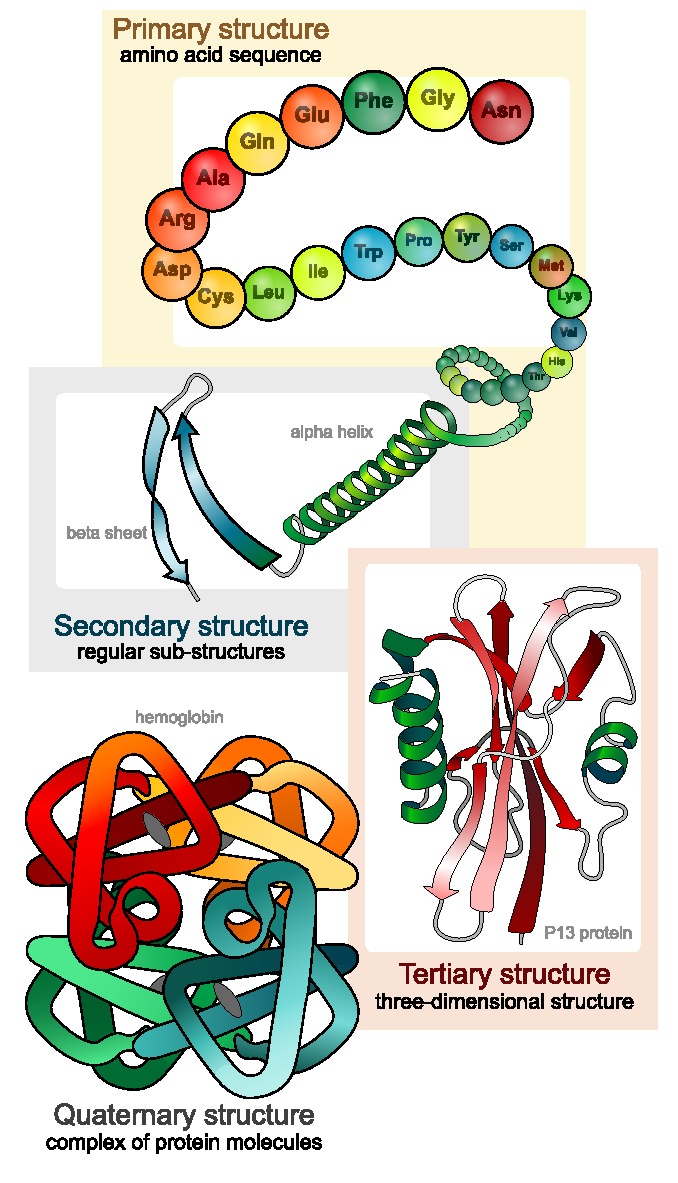
\includegraphics[width=0.6\linewidth]{files/struclevels_alt-0651e6addf2ddae34e55d1fbb7a283cd.pdf}
\caption[]{The four levels of protein structure.
Credits: \href{https://creativecommons.org/publicdomain/zero/1.0/}{CC0 1.0} \cite{struclevels_alt_2008}.}
\label{struclevels_alt}
\end{figure}

The structure of a protein is critical for its function.
For example, in an enzyme, the active site must be in the correct structure to be able to bind the substrate.
Other proteins might bind proteins (and influence their activity) or bind DNA (and regulate gene expression).
Additionally, some proteins are secreted from the cell or might function within the cell membrane.
Finally, proteins are often modified after protein synthesis (see Translation), called post-translational modification.
These modifications can be important for protein function.


\bigskip
\centerline{\rule{13cm}{0.4pt}}
\bigskip

\subparagraph{Primary structure}

In a protein, amino acids are connected by covalent bonds, called peptide bonds.
A peptide bond connects one amino acid's carobxyl group and the next amino acid's amino group (Figure~\ref{peptidebond}).
The sequence of amino acids linked by peptide bonds is called the \textbf{primary structure}.
The protein sequence is determined by the gene sequence encoding the protein.
The continuous chain of atoms along the protein is also called the \textbf{backbone}, it consists of the three backbone atoms (nitrogen, C\textsubscript{$\alpha$}, carbon).

\begin{figure}[!htbp]
\centering
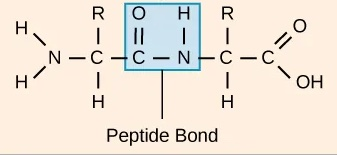
\includegraphics[width=0.4\linewidth]{files/peptidebond-e8f0cd028cafbd2c5d54433c3d2dae1a.jpg}
\caption[]{A peptide bond connecting two amino acids.
Credits: \href{https://creativecommons.org/licenses/by/4.0}{CC BY 4.0} \cite{proteins_2018}.}
\label{peptidebond}
\end{figure}

Each protein has a free amino group on one end, called the \textbf{N terminus}.
The other end has a free carboxyl group, called the \textbf{C terminus}.

\begin{framed}
\textbf{Note 1.1: possible polypeptide chains}\\
As there are 20 distinct amino acids, there can be a huge number of different polypeptide chains, i.e., 20\textsuperscript{n} for a polypeptide of length n.
Most of these potential sequences do not adopt a stable conformation, thus only a tiny fraction of these possibilities exist in nature.
\end{framed}


\bigskip
\centerline{\rule{13cm}{0.4pt}}
\bigskip

\subparagraph{Secondary structure}\label{chapter1_secondary_structure}

Secondary structures are local conformations in the protein that are stabilized by hydrogen bonds between backbone atoms.
We distinguish the regular helices (i.e., alpha helix - $\alpha$-helix) and sheet structures (i.e., beta sheet - $\beta$-sheet) (Figure~\ref{secstructure_alt}) and irregular turns.

\textbf{$\alpha$-helices} are stabilized by hydrogen bonds between the oxygen atom in the C group in one amino acid, and the hydrogen in the N group of the amino acids that is four amino acids farther along the chain.
Every helical turn has 3.6 amino acids residues and the side chains stick out of the helix.

$\beta$-pleated sheets (short: \textbf{$\beta$-sheets}) consist of $\beta$-strands, where the R groups extend above and below the strands.
The strands have a direction determined by the N- and C-terminus of the protein and are usually depicted as an arrow pointing towards the C-terminus.
Depending on the direction, strands can align parallel or antiparallel to each other.

% :::{figure} images/chapter1/secstructure.jpg
% :alt: Secondary structure elements
% :width: 80%
% :name: secstructure
% 
% α-helices and β-sheets are stablized by hydrogen bonds between the backbone of proteins, i.e., the side chains are not involved.
% The hydrogen bonds form between the oxygen atom in the C group in one amino acid and the hydrogen in the N group.
% Black = carbon, white = hydrogen, blue = nitrogen, and red = oxygen. Credits: Rao, A., Tag, A. Ryan, K. and Fletcher, S. Department of Biology, Texas A&M University.
% :::
% #% Unable to use figure secstructure due to copyright.

\begin{figure}[!htbp]
\centering
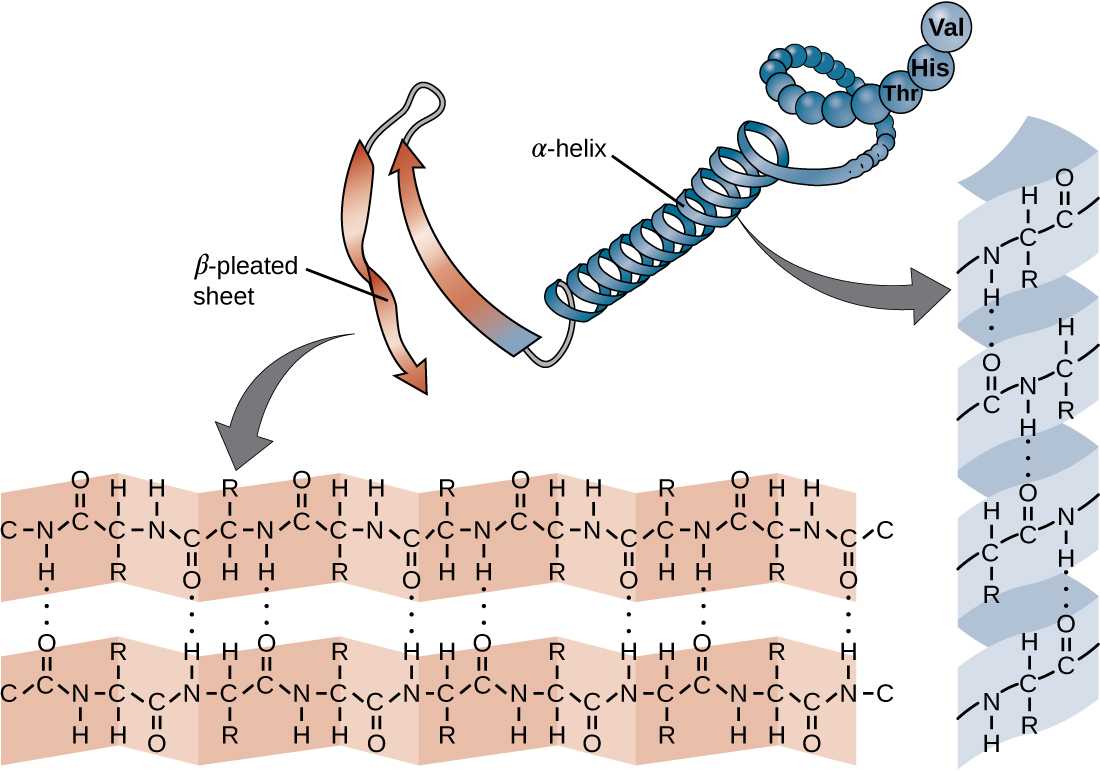
\includegraphics[width=0.8\linewidth]{files/secstructure_alt-aad81a4d80b9af3bc2a1f645520d36e5.jpg}
\caption[]{$\alpha$-helices and $\beta$-sheets are stablized by hydrogen bonds (the dotted lines) between the backbone of proteins, i.e., the side chains are not involved.
The hydrogen bonds form between the oxygen atom in the C group in one amino acid and the hydrogen in the N group.
Credits: \href{https://creativecommons.org/licenses/by/4.0}{CC BY 4.0} modified from \cite{secstructure_alt_nd}.}
\label{secstructure_alt}
\end{figure}

\textbf{Turns} are short secondary structure elements that are stabilized by hydrogen bonds between amino acids that are 1 to 5 peptide bonds away.
The most common form are $\beta$-turns, which connect antiparallel $\beta$-strands.

\begin{framed}
\textbf{Note 1.2: Secondary structure amino acid preference}\\
Although secondary structure elements are formed by hydrogen bonds between the backbone, certain amino acids are favoured in secondary structures and others are disfavoured.
For example, methionine, alanine, leucine, and glutamic acid are favoured in $\alpha$-helices, whereas proline, glycine, and tyrosine are disfavoured.
Also, valine, isoleucine, tyrosine, cysteine, tryptophan, phenylalanine, and threonine are more frequently found in $\beta$-sheets, compared to $\alpha$-helices.
In turns, glycine, asparagine, proline, and serine are preferred.
These preferences are used to predict secondary structure elements in proteins (see chapter~4).
\end{framed}

The peptide bond is very rigid and planar, i.e., it cannot rotate to form the elements of protein structure.
However, the N-C\textsubscript{$\alpha$} and the C\textsubscript{$\alpha$}-C bonds can freely rotate, being only limited by the size and properties of the R-groups.
The 3D shape of the polypeptide backbone is thus determined by two \textbf{torsion angles}:
phi ($\varphi$) between N and C\textsubscript{$\alpha$} and psi ($\psi$) between C\textsubscript{$\alpha$} and C (Figure~\ref{phipsi_alt}A).
Although $\varphi$ and $\psi$ can rotate in principle, steric hindrance prevents certain combinations of angles, i.e., the bulkiness of the R-groups restricts the possible conformations.
Thus, certain combinations of $\varphi$ and $\psi$ are preferred.
We can plot the combinations of $\varphi$ and $\psi$ in a protein, in a so-called \textbf{Ramachandran plot} (Figure~\ref{phipsi_alt}B).

The regular secondary structure elements ($\alpha$-helix and $\beta$-sheet) contain consecutive amino acids with similar ($\varphi$,$\psi$) values.
These regions are typically highly populated in a Ramachandran plot.
Thus, the Ramachandran plot can be used to assess how plausible a predicted protein structure is.

% :::{figure} images/chapter1/phipsi.jpg
% :alt: Phi, psi, and Ramachandran plot
% :width: 70%
% :name: phipsi
% 
% A) Peptide bond, φ, and ψ.
% B) A typical Ramachandran plot. The regions marked "core" do not have any steric hindrance.
% Yellow areas are generally allowed.
% White areas represent conformations that are generally sterically unfavorable.
% Credits: {cite}`phipsi_2014`.
% :::
% #% Unable to use figure phipsi due to copyright.

\begin{figure}[!htbp]
\centering
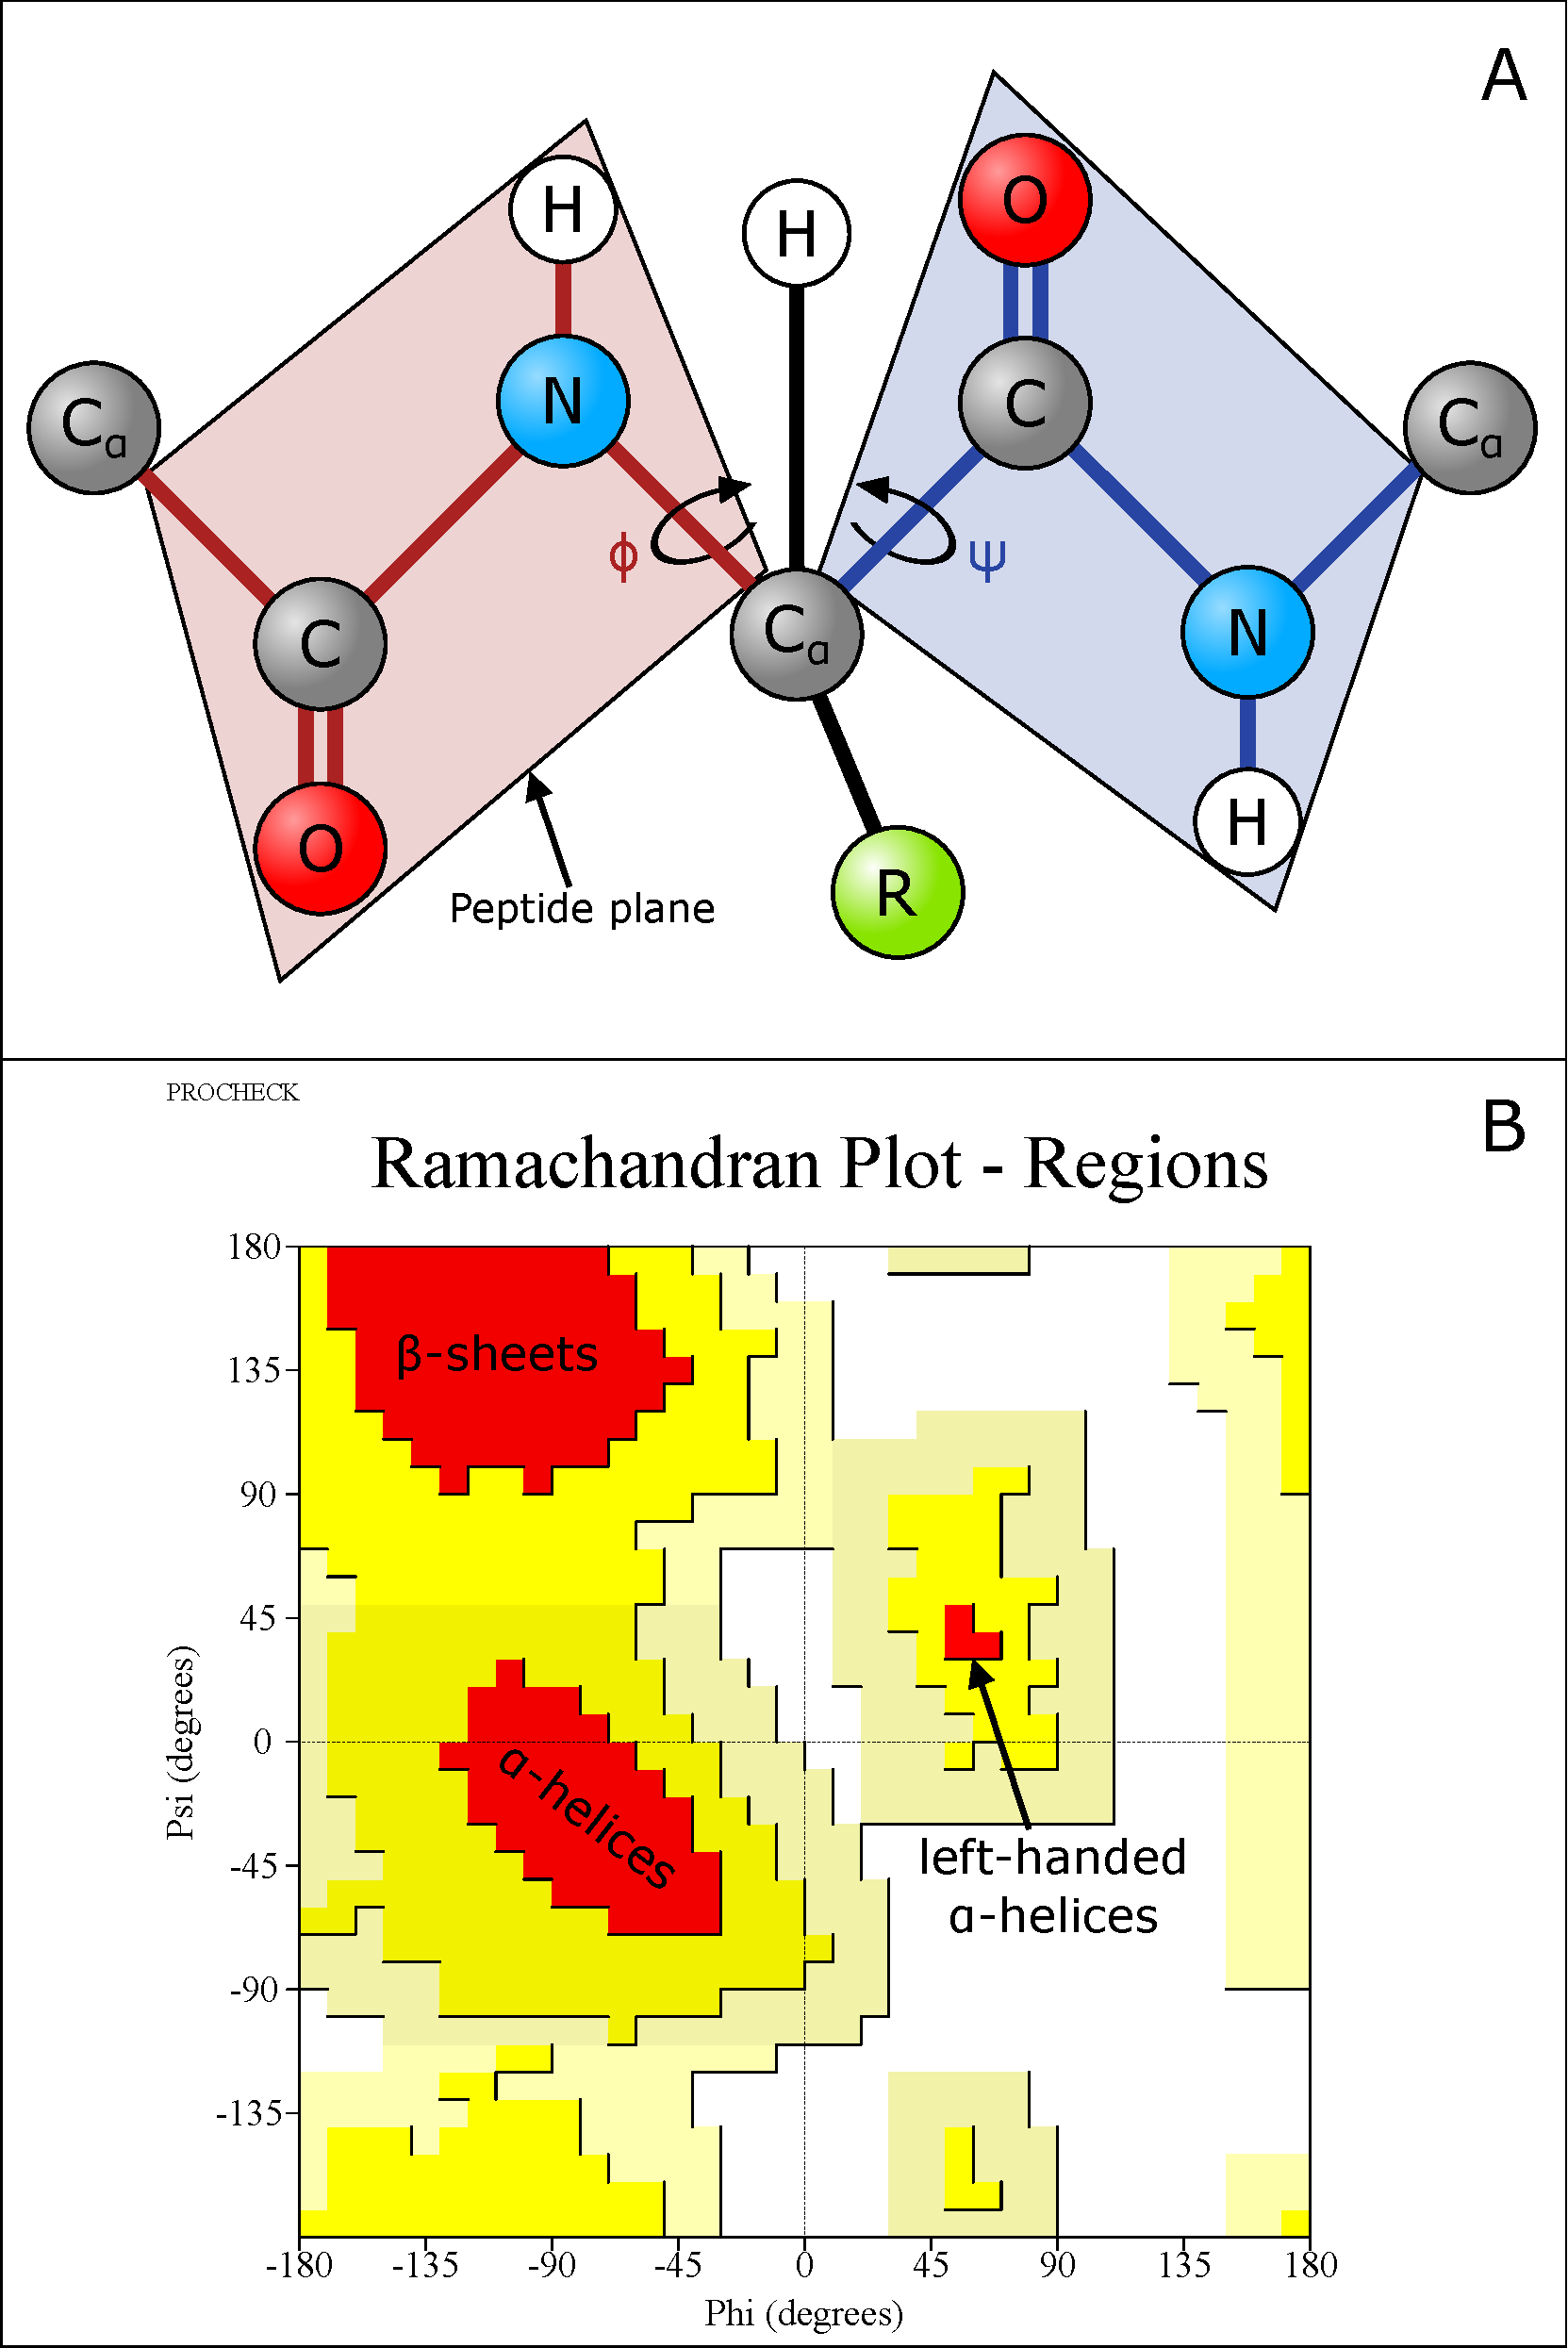
\includegraphics[width=0.5\linewidth]{files/phipsi_alt-4119b9376f7dfe565d87043a7e7a0417.pdf}
\caption[]{A) The $\varphi$, and $\psi$ torsion angles of a polypeptide chain. Credits: \href{https://creativecommons.org/licenses/by-nc/4.0/}{CC BY-NC 4.0} \cite{own_1_2024}.
B) A typical Ramachandran plot. The red regions marked do not have any steric hindrance, yellow areas represent conformations that have steric hindrance, light yellow areas represent conformations that are generally sterically unfavorable, and white areas do not have any allowed conformations.
Credits: Ramachandran plot modified from \href{https://www.ebi.ac.uk/thornton-srv/software/PROCHECK/index.html}{PROCHECK} \cite{procheck_1993}.}
\label{phipsi_alt}
\end{figure}

\begin{framed}
\textbf{See Also}\\
An illustrative animation on $\varphi$ and $\psi$.
\end{framed}


\bigskip
\centerline{\rule{13cm}{0.4pt}}
\bigskip

\subparagraph{Tertiary structure}

The tertiary structure of a protein describes the complete folding of an entire polypeptide chain.
In contrast to the secondary structure, the tertiary structure of a protein involves interactions between the amino acid's side chains that can occur at short-range and long-range (Figure~\ref{terstructure}).
Thus, the chemical properties of the amino acids are very important for the tertiary structure.
Different types of interactions stabilize the tertiary structure:

\begin{itemize}
\item Hydrogen bonds involving polar amino acids.
\item Ionic bonds between positively and negatively charged amino acids.
\item Hydrophobic R groups that tend to lie in the protein's interior, stabilized by hydrophobic interactions.
\item Disulfide bonds (i.e., covalent bonds between cysteines).
\end{itemize}

\begin{figure}[!htbp]
\centering
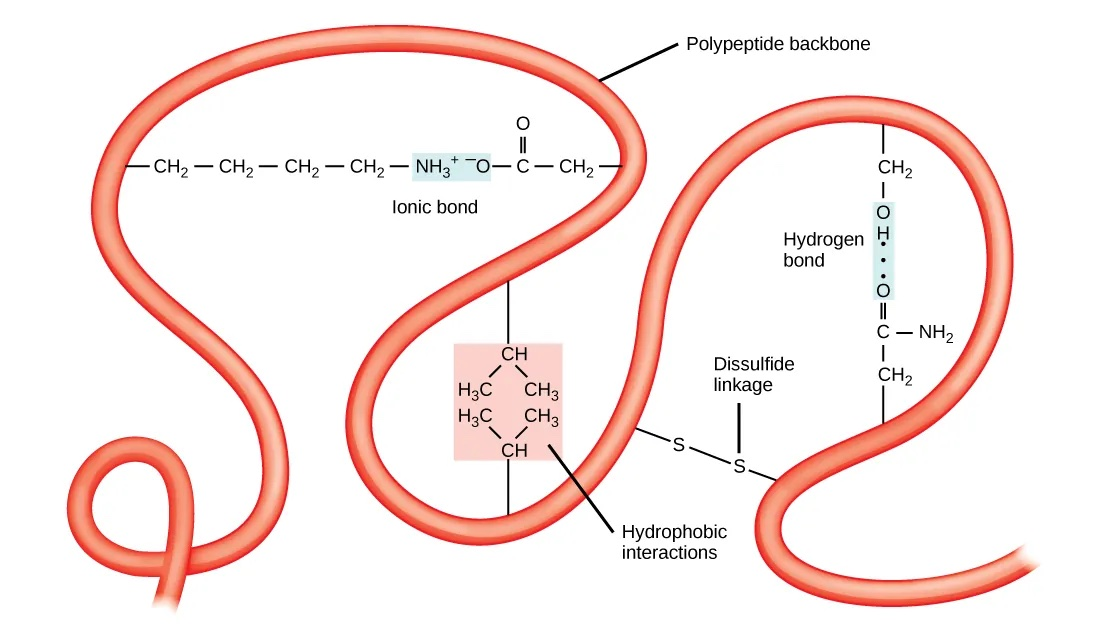
\includegraphics[width=0.8\linewidth]{files/terstructure-4b7f78306caf16f9c7283bc23fe4a55b.jpg}
\caption[]{Chemical interactions that stabilize the tertiary structure of proteins.
Credits: \href{https://creativecommons.org/licenses/by/4.0}{CC BY 4.0} \cite{proteins_2018}.}
\label{terstructure}
\end{figure}

\begin{framed}
\textbf{Note 1.3: Denaturation}\\
The noncovalent bonds that stabilize the protein structure are broken at high temperature.
Thus, most proteins unfold above about 60°C.
This process is called denaturation and is generally irreversible.
When proteins denature, they lose their function.
\end{framed}

\textbf{Domains} are distinct functional and/or structural units in a protein and are typically 50 to 350 amino acids long.
Usually, a domain is responsible for a particular function or interaction, contributing to the overall role of a protein.
A domain can exist in different contexts with other domains (Figure~\ref{domains}).
In a multidomain protein, each domain folds independently of the others.

\begin{figure}[!htbp]
\centering
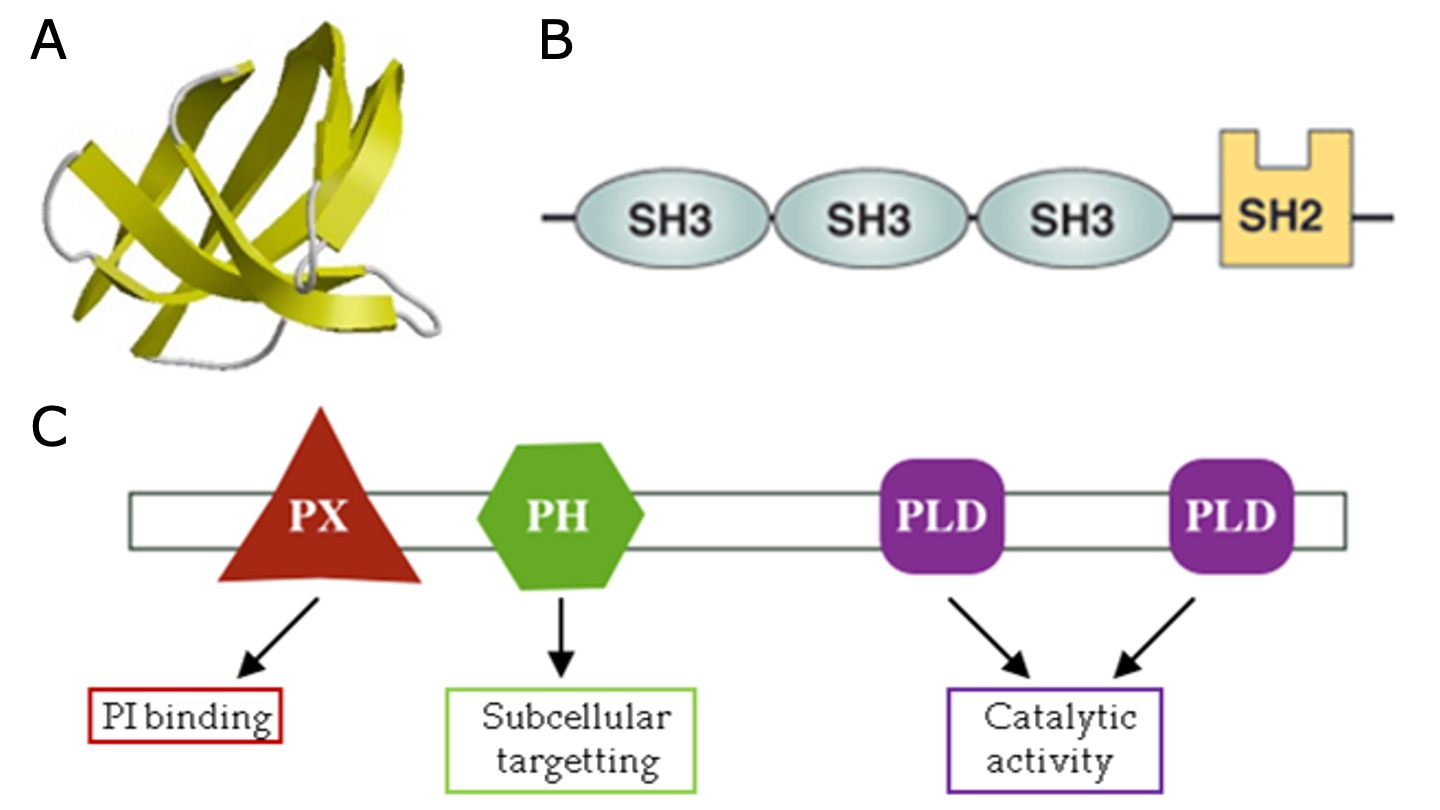
\includegraphics[width=0.7\linewidth]{files/domains-7cca8056e5affaf9aa34f387f50bc335.jpg}
\caption[]{A) Example of an Src homology 3 (SH3) domain that is involved in protein-protein interaction. SH3 domains occur in a diverse range of proteins with different functions.
B) The cytoplasmic protein Nck contains multiple SH3 domains.
C) Domain composition of phospholipase D1, which has multiple functional domains that contribute to its overall function.
Credits: \href{https://creativecommons.org/licenses/by/4.0}{CC BY 4.0} \cite{domains_2023}.}
\label{domains}
\end{figure}


\bigskip
\centerline{\rule{13cm}{0.4pt}}
\bigskip

\subparagraph{Quaternary structure}

Finally, individual folded polypeptides can interact to form \textbf{protein complexes}, also called quaternary structures.
The quaternary structure is stabilized by the same types of interactions as the tertiary structure.
The difference is that the amino acids involved belong to different polypeptides.

Many functional proteins are composed of multiple subunits, they are also called \textbf{oligomers} (Figure~\ref{oligomers}).
The subunits can originate from the same protein sequence (called a homomer) or from different sequences (called a heteromer).
Proteins consisting of two subunits are also called dimer.

\begin{figure}[!htbp]
\centering
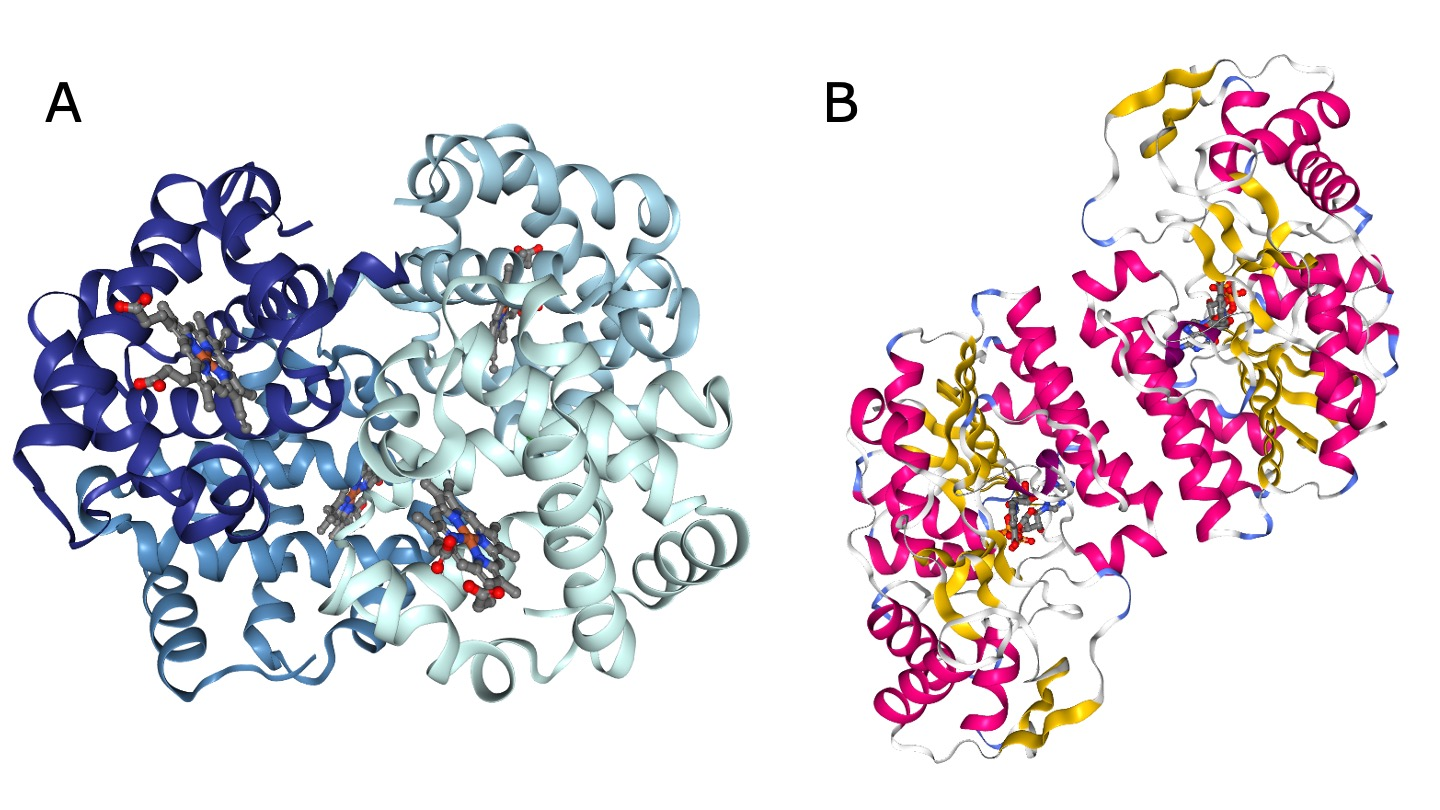
\includegraphics[width=0.7\linewidth]{files/oligomers-eac46cb02a81a2c53b32d003ffc2198f.jpg}
\caption[]{Examples of oligomers.
A) Myoglobin, a heteromer of four subunits (PDB structure 1HV4 colored by chain). Credits: \citet{rcsb_2000, oligomers_a_2001, ngl_2018}.
B) UDP-galactose 4-epimerase, a homodimer (PDB structure 1EK5 colored by secondary structure). Credits: \citet{rcsb_2000, oligomers_b_2000, ngl_2018}.}
\label{oligomers}
\end{figure}


\bigskip
\centerline{\rule{13cm}{0.4pt}}
\bigskip

\subparagraph{Substitutions}\label{chapter1_substitutions}

Mutations in the gene sequence can lead to changes in the primary structure of the protein, e.g., a substitution of one amino acid by a different one.
Often, such substitutions still lead to highly similar protein structures that perform a similar or even the same function, especially when the exchanged amino acids have similar chemical properties.
Nevertheless, single amino acid substitutions can have severe consequences.
A prominent example is sickle cell anemia, where a substitution of valine to glutamic acid in hemoglobin $\beta$ results in a structural change that leads to a distortion in red blood cells (Figure~\ref{sicklecell}).

\begin{figure}[!htbp]
\centering
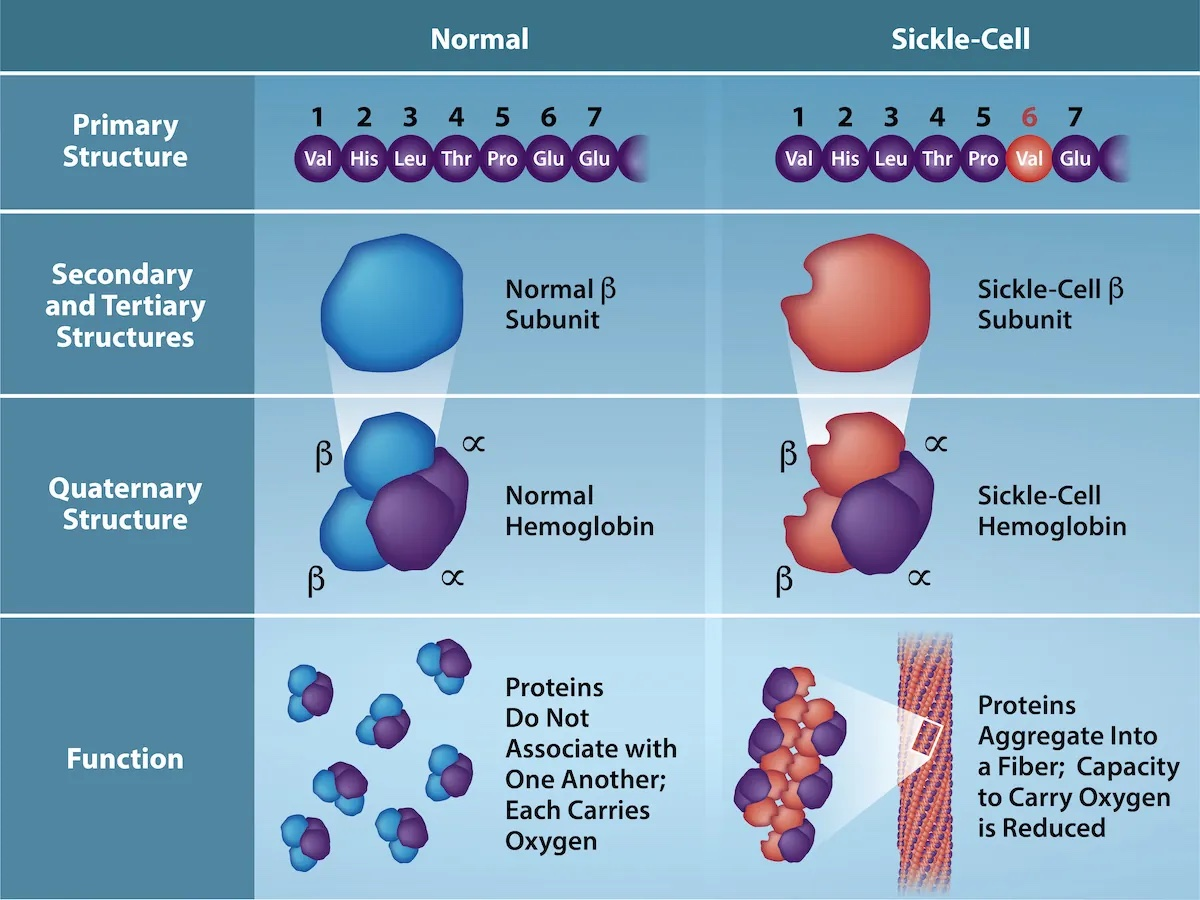
\includegraphics[width=0.7\linewidth]{files/sicklecell-9c221211df6604b37609733b9d82c043.jpg}
\caption[]{Consequences of a substitution in hemoglobin $\beta$ resulting in sickle cell anemia.
Credits: Rao, A., Tag, A. Ryan, K. and Fletcher, S. Department of Biology, Texas A\&M University.}
\label{sicklecell}
\end{figure}

% #% Figure sicklecell is credited but the image is not found on a specific webpage. Is showing credits enough? - Similar to Pearson imagery (Campbell Biology 11th edition Figure 5.19).


\bigskip
\centerline{\rule{13cm}{0.4pt}}
\bigskip

\subparagraph{Visualization}

There are many styles to view protein molecular structures. Some styles focus on detailed chemical structure, others are targeted at the protein surface.
For some examples see Figure~\ref{protrep}.

\begin{figure}[!htbp]
\centering
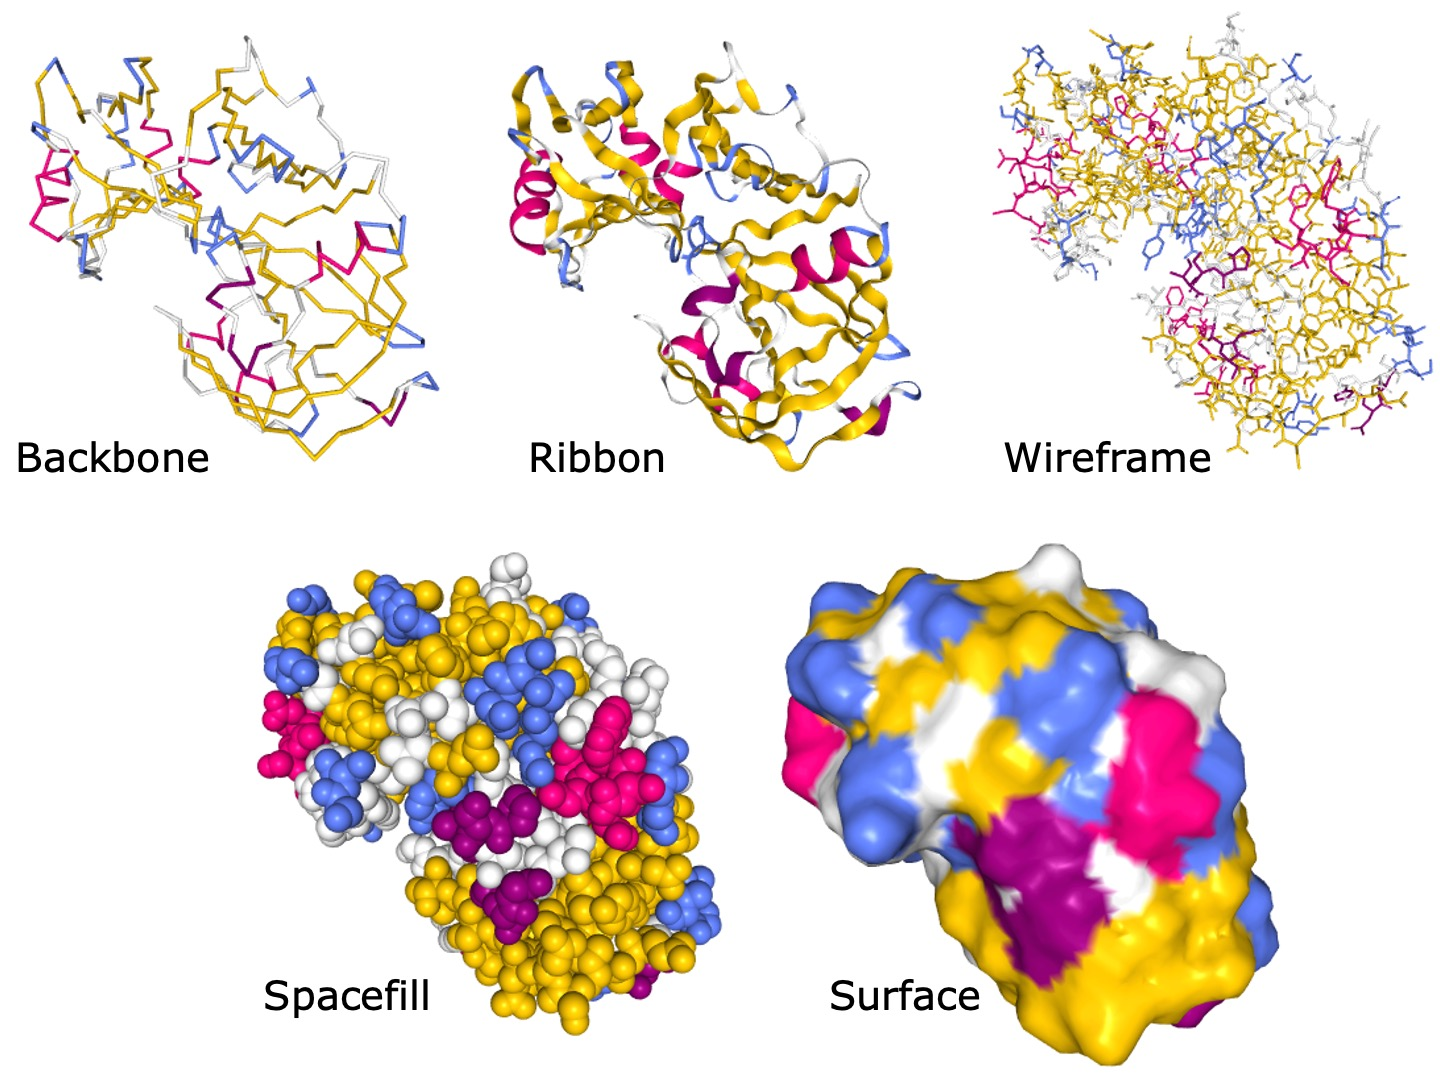
\includegraphics[width=0.6\linewidth]{files/protrep-dbcbffe70f8b8a99767b7579c1bd83d0.jpg}
\caption[]{Different representations of the PDB structure 5PEP generated with NGL. Credits: \citet{rcsb_2000, protrep_1990, ngl_2018}.}
\label{protrep}
\end{figure}

% #% The citation above does not end up in alphabetical order. This is probably caused by ngl_2018 being referenced earlier in the markdown than protrep_1990. Not sure how to fix without adopting a custom inline citation reference style.

\begin{framed}
\textbf{See Also}\\
Most of the figures in this section are taken from \href{https://openstax.org/books/biology-2e/pages/3-4-proteins}{OpenStax}, where you can also find more information on proteins.
\end{framed}


\bigskip
\centerline{\rule{13cm}{0.4pt}}
\bigskip

\subsubsection{Genome annotation}\label{chapter1_genome_annotation}

Genome annotation is the process of deciphering what information is encoded in an organism's DNA.
It is an ongoing effort in organisms with known genome sequences.
Even moreso, genome annotation is a critical step in acquiring biological insights from newly sequenced genomes.
Given the large size of any genome, automated procedures are used to identify various genomic elements such as genes, regulatory regions, transposable elements, or other non-coding elements.
Each of these bioinformatic procedures typically focuses on identifying one type of element, and as such a complete genome annotation project can be thought of as a pipeline of various procedures.
The following section describes the most common steps in genome annotation.

\begin{framed}
\textbf{Note 1.4: Alignment algorithms}\\
Several steps in the genome annotation process make use of algorithms that can search or align biological sequences, for example the BLAST algorithm.
\href{/chapter2}{Chapter 2} covers sequence alignment and search in greater detail.
For now, it is sufficient to know that these algorithms can quickly search very large collections of biological sequences to identify sequences that look similar (what we mean \textit{exactly} by `similar' is also part of \href{/chapter2}{chapter 2}).
\end{framed}

\paragraph{Repeat masking}\label{Chapter1_repeat_masking}

Repeat masking involves the identification and masking (hiding) of repetitive sequences within a genome.
It is an essential first step in annotating most genomes because repetitive sequences can pose significant challenges in genome annotation.
Masking repeats generally improves:

\begin{itemize}
\item Accuracy: repetitive elements can be mistakenly annotated as genes or other functional elements, leading to inaccurate predictions and interpretations of the genome.
\item Computational efficiency: identifying and processing repetitive sequences can be computationally intensive.
However, masking these repetitive regions reduces the computation time of all downstream analyses.
\item Biological relevance: repetitive sequences are usually not involved in the coding of proteins of interest.
Therefore, focusing on non-repetitive regions is a smart choice in understanding the genes and regulatory elements that drive biological processes.
\end{itemize}

Most repeat masking workflows work by first compiling (or using a precompiled) `repeat library': a collection of known repetitive elements that have previously been characterized.
Subsequently, the genome to be annotated is compared against this repeat library using various computational algorithms, such as BLAST or RepeatMasker.
When a match is found, the corresponding region in the genome is `masked' or annotated as a repetitive element.
This means that these regions are excluded from further analysis or labeled as repetitive.

\paragraph{Gene prediction}\label{Chapter1_gene_prediction}

The process of finding protein coding genes differs between prokaryotic and eukaryotic genomes.
In both cases the aim is to find open reading frames (ORFs): contiguous stretches of DNA that encode proteins.
However, since RNA splicing (Figure~\ref{splicing}) is almost absent in prokaryotic genomes, prokaryotic ORFs can be found directly in the genomic DNA.
As a result, simply enumerating all possible ORFs in a genome is a common step in prokaryotic genome annotation.
In contrast, ORFs in eukaryotic genomes are found on \textit{mature} mRNAs. As such, all eukaryotic gene prediction methods take splicing into account, thereby greatly increasing their computational complexity.
Both prokaryotic and eukaryotic gene prediction typically can be classified as either evidence based prediction or ab initio prediction, both will be explained below.

\subparagraph{Evidence based prediction}

This data-driven approach uses existing and newly generated data to get hints on what regions of a genome encode genes.
Depending on the type of data, these predictions have more or less predictive power.
Some commonly used evidence types are:

\begin{itemize}
\item RNA-sequencing data: the most direct form of evidence for what regions of the genome are transcribed.
As such, RNA-sequencing (often abbreviated to RNA-seq) `reads' often provide the best form of evidence in identifying splice sites in eukaryotes.
Note that not all transcribed RNA will be translated into proteins, and that therefore not all RNA-sequencing reads are evidence for protein coding genes.
Distinguishing between protein-coding and non-coding RNA is not always trivial.
\item Homology evidence: Aligning DNA or protein sequences of known genes (from other organisms) is valuable evidence in finding coding regions of the genome.
Due to the redundancy in the genetic code, it is not trivial to correctly identify splice sites when aligning protein sequences to a genome.
Homology evidence from closely related organisms leads to higher quality predictions than evidence from distantly related organisms.
\item Whole-genome alignments: this approach uses the annotated genome of a closely related organism to directly identify coding regions in a novel genome.
For example: whole-genome alignment of mouse and human genomes reveals that large parts of mouse chromosome 2 are homologous to human chromosome 20.
The alignment procedure results in a direct 1-to-1 mapping of mouse and human genome coordinates, and as such annotation coordinates can be transferred between genomes.
\end{itemize}

\subparagraph{Ab initio prediction}

\begin{quote}
\textit{Ab initio} (latin): from first principles, from the beginning
\end{quote}

These methods rely on statistics to learn a predictive model from a known annotated genome.
Various forms of ab initio models exist, and whereas implementation details differ, most follow a similar line of reasoning.
For now, we will stick to a high level description.
All ab initio models scan through a DNA sequence and at each position give a score for a specific type of annotation.
In addition, they often take their genomic context into account.
For example, the probability of a protein-coding annotation on a nucleotide A is high when the next two observed nucleotides are T and G, producing the ATG start-codon methionine.
In addition, most methods also take the \textit{predicted annotation} of the genomic context into account.
For example: the probibility that ATG actually codes for a start codon is much higher if we can predict an in-frame stop codon.
In eukaryotic genome prediction these models become quite complex because they have to include splice sites in all three reading frames.
How \textit{exactly} a model decides what annotation score to give to which nucleotide is part of the model architecture and parameterization.
In all cases, the model parameters are chosen to accurately reproduce a known genome annotation.
If sufficient data is used to learn the model parameters, it is assumed that these models can be used to predict annotations on novel genome sequences.
Like homology-based prediction, this model-based approach works best for closely related organisms. In the past, almost all ab initio prediction methods were formulated as hidden Markov models (HMMs) (see Note 1.5). Examples of tools implementing HMM based ab initio prediction are SNAP, GeneMark, and Augustus. With the availability of more high quality data (genome sequences and accompanying annotations), approaches based on deep learning and generative AI have proven to frequently perform better than HMM based approaches.

\begin{framed}
\textbf{Note 1.5: Hidden Markov models (HMMs)}\\
Hidden Markov models (HMMs) are useful for the statistical modelling of general sequence characteristics. As such they find widespread adoption in bioinformatics to study biological sequences. Providing a full technical description of all aspects of HMMs is outside of the scope of this book. Here we will stick to a somewhat simplistic description to provide a first introduction.

A hidden Markov model can be used to predict some unobserved labelling across a sequence of observations. For example: in genome annotation, coding and non-coding regions of a genome can be treated as an unobserved characteristic, where the nucleotides are the sequence of observations. As such, `hidden' refers to the \textit{unobserved labelling}. In addition, `Markov' refers to some useful statistical assumptions on the nature of independence between observations and labellings that enable efficient computation.

More formally, the unobserved labellings are referred to as the `hidden states', and every hidden state contains some probabilities of observing our sequence of interest, called the `emission probabilities'. To complete our HMM definition, we define `transition probabilities' between hidden states.

The combination of hidden states, emission probabilities, and transition probabilities enable asking questions such as `given my current observation and a certain label of my previous observation, what is the most likely label for my current observation?'. In the context of genome annotation this would translate to for example `given that I see a stop-codon, and that my previous label was coding sequence, what is my current most likely label?', the answer to which would be `non-coding' (See Figure~\ref{coding_hmm}).

\begin{figure}[!htbp]
\centering
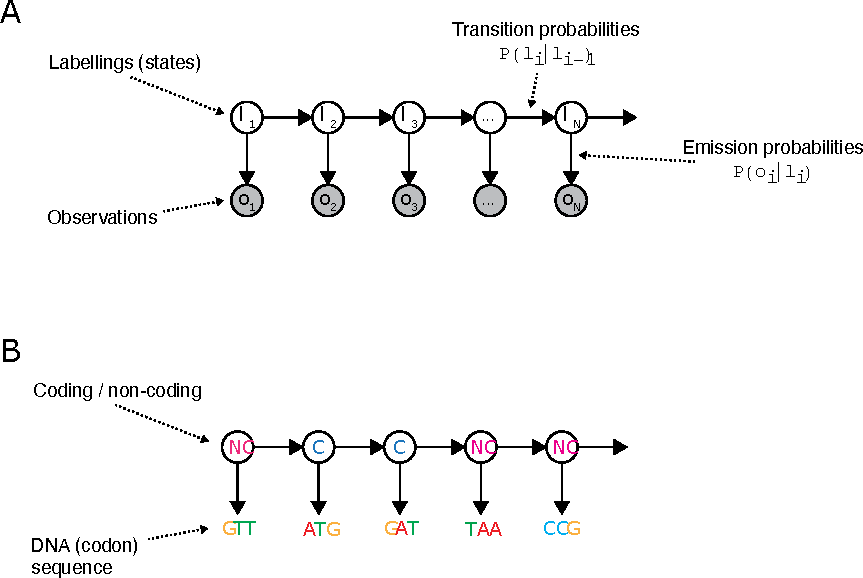
\includegraphics[width=1\linewidth]{files/coding_hmm-22db191de15f76bd6deb9e5904ea2580.pdf}
\caption[]{\textbf{A}: Graphical representation of a general hidden Markov model. Shaded circles indicate observations, white circles indicate unobserved labellings (hidden states). Black arrows indicate transition probabilities between hidden states, and emission probabilies for observations from hidden states. Note that there are no arrows between observations! This is one of the properties of HMMs that enable efficient computation. \textbf{B}: A (simplified) HMM variant that labels a sequence of DNA codons as either coding or non-coding. Real-world gene predicition HMMs use a more elaborate structure with more hidden states, and six-frame representations of the DNA.
Credits: \href{https://creativecommons.org/licenses/by-nc/4.0/}{CC BY-NC 4.0} \cite{own_1_2024}.}
\label{coding_hmm}
\end{figure}

\href{/chapter2}{Chapter 2} and \href{/chapter4}{Chapter 4} cover various other applications of HMMs in bioinformatics, such as defining and prediction sequence domains, or transmembrane properties of proteins.
\end{framed}

\paragraph{Evidence/prediction integration}

From the previous sections it has now become clear there are several ways of predicting what the genes in a genome look like.
Since these various approaches almost never agree exactly in their predictions, a final step in genome annotation is evidence and prediction integration.
Typically a weighted consensus approach is used: each individual source of evidence is given a weight representing how much it should influence the final decision, after which a majority vote decides what the annotation should look like.
Typically RNA-seq evidence gets a high weight, and various forms of homology evidence can be weighted depending on how closely related they are to the genome of interest.

\paragraph{Functional annotation}\label{chapter1_functional_annotation}

So far, all described steps in the genome annotation process have dealt with what genes look like on a structural level.
To gain biological insight, the next step is to assign functional annotations to the predicted genes.
This functional annotation step consists of using various sequence alignment and search tools to find sequences with a known function/description and to transfer the information of the known gene to the predicted gene.
Several databases of high-quality known functions are often used, which are described in more detail in the next section of this chapter.
In Chapter~2 we will learn about approaches how to search these databases efficiently.

\begin{framed}
\textbf{Note 1.6: Visualizing gene structure}\\
\textbf{Gene models}: the genomic structure of a gene (often referred to as a gene `model') is typically visualized by a set of lines and rectangles with predefined meaning.

\begin{figure}[!htbp]
\centering
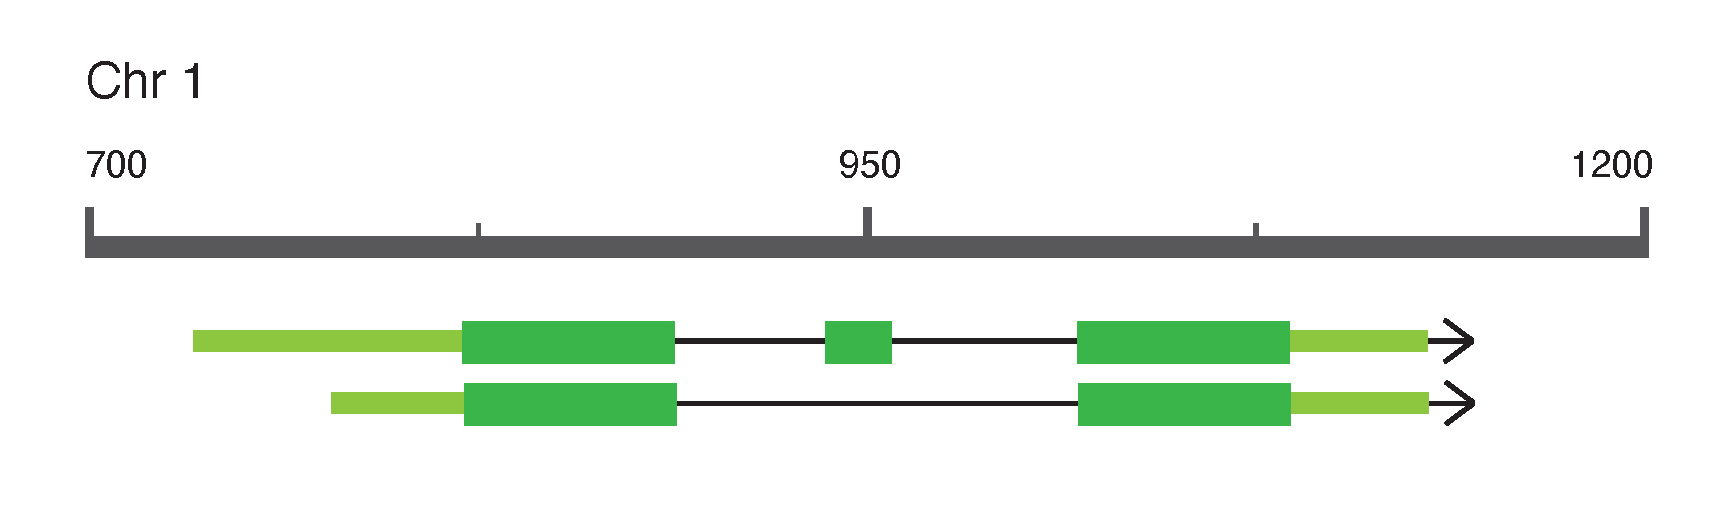
\includegraphics[width=1\linewidth]{files/genemodel-7bb5f6683cb808b770f42927d7e7aacb.png}
\caption[]{An example gene model.
Various visualization conventions can be identified: boxes represent genomic regions that are transcribed.
Boxes are exons, lines between boxes are introns. Narrow boxes (sometimes with a lighter color) are untranscribed regions (UTRs), wider boxes (sometimes darker colored) are coding sequence regions (CDS).
The arrow indicates the direction of transcription.
In this example a gene on chromosome 1 with two splice variants is shown, where the first variant has a slightly longer 5' UTR and an additional CDS exon in between the first and last exons.
Credits: \href{https://creativecommons.org/licenses/by-nc/4.0/}{CC BY-NC 4.0} \cite{own_1_2024}.}
\label{genemodel}
\end{figure}

\textbf{Genome browsers} facilitate interactive visualization of annotations and evidence alignments on genome sequences.
Various implementations exist, but all genome browsers typically provide a linear view of a chromosome that can be scrolled and zoomed.
In addition, various annotation `tracks' can often be toggled, to display for instance known gene structures, RNA sequencing alignments, or homologous protein sequence alignments.
Most visualization elements can be clicked to open pop-up windows with additional information.

\begin{figure}[!htbp]
\centering
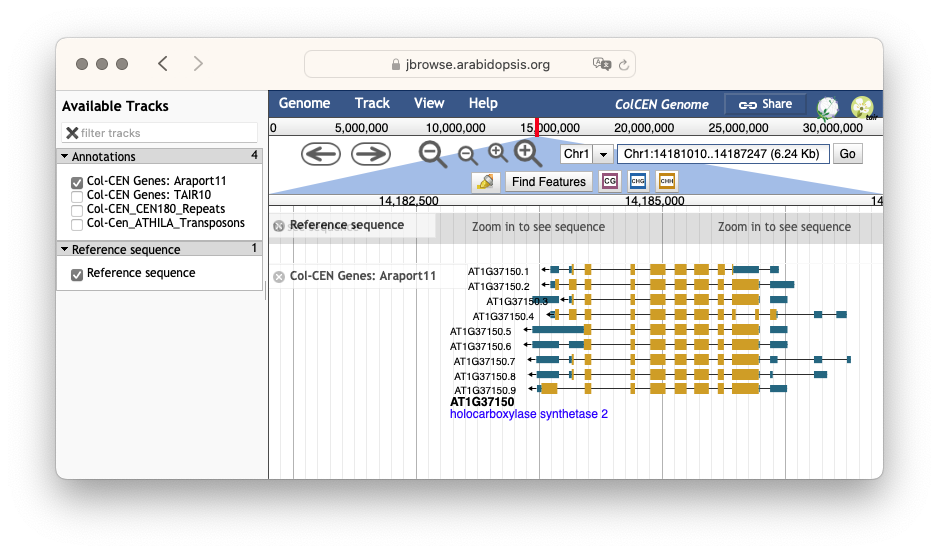
\includegraphics[width=1\linewidth]{files/jbrowse-54f15198e78cd826afaaf0266ba943cb.png}
\caption[]{A screenshot of the JBrowse genome browser showing \textit{Arabidopsis thaliana} chromosome 1 with a gene that has multiple splice variants. Credits: \cite{jbrowse_2016}.}
\label{jbrowse}
\end{figure}
\end{framed}


\bigskip
\centerline{\rule{13cm}{0.4pt}}
\bigskip

\subsubsection{Databases}\label{chapter1_databases}

\paragraph{Introduction}

Databases are at the core of bioinformatics.
In all analyses, we integrate pre-existing data and we need to access this data.
The journal Nucleic Acids Research publishes an entire issue in the beginning of each year on new and updated databases.
The list of these databases can also be accessed \href{https://www.oxfordjournals.org/nar/database/c}{online}.

Computer scientists have developed different kinds of databases.
One example are relational databases, which can be queried by \textbf{SQL} (structured query language) and which perform well for data that is processed computationally.
Another example are \textbf{XML} (extended markup language) databases which store data in specified well-structured XML files.
Nevertheless, most databases for biological sequence data use \textbf{flat file databases}, where the data is saved in structured text files.
This data can be manipulated in a text editor without requiring an additional program for database management, and they can be easily exchanged between scientists.
On the downside, searching them has a lower performance.
This is why they are often indexed, i.e., they contain an \textbf{index} of keywords, similar to a glossary in a book.

Depending on the kind of data included, we distinguish different kinds of biological databases:

\begin{itemize}
\item \textbf{Primary databases} contain primary sequence information from experimentally derived data that is directly submitted by the scientists that generated the data.
\item \textbf{Secondary databases} provide the results of analyses of the information in primary databases.
\end{itemize}

Each entry in a database has a unique \textbf{accession number}.
This number is permanent and provides an unambiguous way to link to the entry.
The information that the accession refers to should not change.
To still allow updates to an entry, the accession number can contain a \textbf{version}, usually after a dot.
For example, NC\_003070.9 is the latest version (version 9) for \textit{Arabidopsis thaliana} chromosome 1 in RefSeq.

Database entries often link to each other via \textbf{cross links}.

\begin{framed}
\textbf{See Also}\\
\href{https://www.ncbi.nlm.nih.gov/pmc/articles/PMC5104318/}{Ten Simple Rules for Developing Public Biological Databases} contains additional reading material on what it takes to properly maintain a public database service.
\end{framed}


\bigskip
\centerline{\rule{13cm}{0.4pt}}
\bigskip

\paragraph{GenBank}

\href{https://www.ncbi.nlm.nih.gov/genbank/}{GenBank} is a popular primary database for nucleotide sequences and is based at the \href{https://www.ncbi.nlm.nih.gov/}{NCBI} (National Center for Biotechnology Information).
A GenBank release usually occurs every two months and the most recent \href{https://www.ncbi.nlm.nih.gov/genbank/release/current/}{release} from the 15\textsuperscript{th} of December 2023 contains {\textasciitilde}250 million sequences and additionally {\textasciitilde}3.7 billion WGS (whole genome shotgun) records.
The latter are genome assemblies or genomes that were not yet completed.
The complete database is available for download via FTP, but the most convenient way to access individual entries is via the search on the GenBank website (Figure~\ref{genbank_figure}).

\begin{figure}[!htbp]
\centering
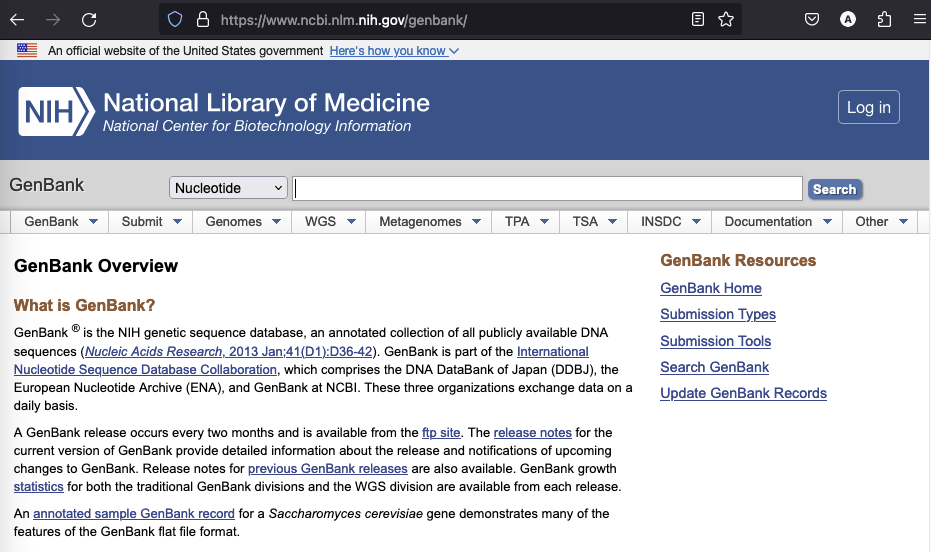
\includegraphics[width=1\linewidth]{files/genbank-f7d7daa5982bc401e1c7f56159ba59fb.png}
\caption[]{A screenshot of the GenBank website. Credits: \cite{genbank_2012}.}
\label{genbank_figure}
\end{figure}

\begin{framed}
\textbf{Additional information}\\
These days, it is required for publication in most peer-reviewed journals that scientists submit their sequence data to GenBank or an associated database, alongside sufficiently informative meta-data that describes how the data was generated.
\end{framed}

Since data is directly submitted to GenBank, the information for some loci can be highly redundant.
The sequence records are owned by the original submitter and cannot be altered by someone else.

\begin{framed}
\textbf{Note 1.7: Database redundancy}\\
`Redundancy' in the context of a database refers to identical data that is present more than once.
Typically, \textit{metadata} is not taken into account when determining redundancy.
Example: two different labs have determined the DNA sequence of a bacterial gene involved in some disease.
The metadata will be different, but the sequence data will be identical, so these two database records are redundant.

NCBI hosts several databases that are classified as `non-redundant', for example \href{https://www.ncbi.nlm.nih.gov/refseq/about/nonredundantproteins/}{RefSeq non-redundant proteins}.
Here, redundancy is defined so that a `non-redundant protein record always represents one exact sequence that has been observed once or many times in different strains or species'.
\end{framed}

Genbank is part of the \href{https://www.insdc.org/}{INSDC} (International Nucleotide Sequence Database Collaboration).
The other two member databases are \href{https://www.ebi.ac.uk/ena/browser/home}{ENA} (European Nucleotide Archive) and \href{https://www.ddbj.nig.ac.jp/index-e.html}{DDBJ} (DNA Data Bank of Japan).
The data submitted to either database is exchanged daily, so all databases contain essentially the same information.


\bigskip
\centerline{\rule{13cm}{0.4pt}}
\bigskip

\paragraph{RefSeq}

The Reference Sequence (\href{https://www.ncbi.nlm.nih.gov/refseq/}{RefSeq}) collection is also hosted at NCBI and contains genomic DNA, transcripts, and proteins.
The aim of RefSeq is to provide non-redundant, curated data.
RefSeq genomes are copies of selected assembled genomes in GenBank.
Additionally, transcript and protein records are generated by several processes:

\begin{itemize}
\item Computation via the \href{https://www.ncbi.nlm.nih.gov/genome/annotation\_euk/}{eukaryotic} or \href{https://www.ncbi.nlm.nih.gov/genome/annotation\_prok/}{prokaryotic} annotation pipeline.
\item Manual curation.
\item Transfer of information from annotated genomes in GenBank.
% #% The eukaryotic and prokaryotic RefSeq links lead to soon to be redundant pages. Not sure what to replace this with.

In contrast to GenBank, RefSeq records are owned by NCBI and can be updated to maintain annotation.
The current release is 222 from the 8\textsuperscript{th} of January 2024 and contains {\textasciitilde}305 million proteins from {\textasciitilde}145,000 organisms.
\end{itemize}

The RefSeq accessions directly provide information on \href{https://www.ncbi.nlm.nih.gov/books/NBK21091/table/ch18.T.refseq\_accession\_numbers\_and\_mole/?report=objectonly}{molecule types}.
For example, \texttt{NC\_} accessions denote complete genomes, \texttt{NP\_} accessions denote proteins in one genome, and \texttt{WP\_} accessions denote proteins in multiple genomes.


\bigskip
\centerline{\rule{13cm}{0.4pt}}
\bigskip

\paragraph{UniProt}\label{chapter1_uniprot}

There is lots of information available for proteins, such as sequence information, domains, expression, or 3D structure.
The aim of the Universal Protein Resource (\href{https://www.uniprot.org/}{UniProt}) is to provide a comprehensive resource for proteins and their annotation.
UniProt contains three databases (Figure~\ref{uniprot}):

\begin{itemize}
\item UniProt Knowledgebase (UniProtKB) - see below.
\item UniProt Reference Clusters (\href{https://www.uniprot.org/help/uniref}{UniRef} - clusters of protein sequences at 100\%, 90\%, and 50\% identity.
\item UniProt Archive (\href{https://www.uniprot.org/help/uniparc}{UniParc} - non-redundant archive of publicly available protein sequences seen across different databases.
\end{itemize}

\begin{figure}[!htbp]
\centering
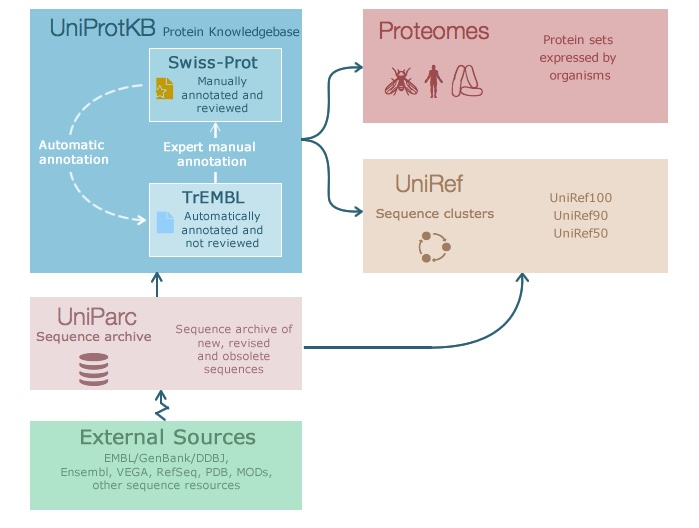
\includegraphics[width=0.7\linewidth]{files/uniprot-93dd5f84ee9208207fa0fe44b574d65a.jpg}
\caption[]{The information flow in Uniprot.
Credits: \href{https://creativecommons.org/licenses/by-nc-nd/4.0/}{CC BY-NC-ND 4.0} \cite{uniprot_2021}.}
\label{uniprot}
\end{figure}

\textbf{UniProtKB} is the central hub for functional information on proteins.
For each protein it contains the core data (such as sequence, name, description, taxonomy, citation) and as much annotation information as possible.
It contains many cross-references to other databases and is generally a very good starting point to find information on a protein.

UniProtKB consists of two sections:

\begin{itemize}
\item \href{https://web.expasy.org/docs/userman.html\#what\_is\_sprot}{Swiss-Prot} - manually-annotated records with information extracted from literature and curated computational analysis.
\item \href{https://web.expasy.org/docs/userman.html\#what\_is\_trembl}{TrEMBL} - automatically annotated records that are not reviewed.
\end{itemize}

UniProtKB is updated every 8 weeks. The current release has {\textasciitilde}570,000 entries in Swiss-Prot and {\textasciitilde}248 million entries in TrEMBL.


\bigskip
\centerline{\rule{13cm}{0.4pt}}
\bigskip

\paragraph{Prosite}\label{chapter1_prosite}

\href{https://prosite.expasy.org/}{Prosite} is a secondary database of protein domains, families, and functional sites.
Some regions in protein families are more conserved than others because they are important for the structure or function of the protein.
Prosite contains motifs and profiles specific for many protein families or domains.
Searching motifs in new proteins can provide a first hint for protein function.

The current release of Prosite from the 24\textsuperscript{th} of January 2024 contains 1311 patterns, 1386 profiles, and 1400 ProRule entries.

A Prosite \textbf{pattern} is typically 10 to 20 amino acids in length.
These short patterns are usually located in short well-conserved regions, such as catalytic sites in enzymes or binding sites.
A pattern is represented as a regular expression, where amino acids are separated by hyphens and \texttt{x} denotes any letter.
Repetitions can also be given as the number of repetitions in brackets.
For example, \texttt{[AC]-x-V-x(4)-\{ED\}} matches sequences that contain the following amino acid sequence: Ala or Cys-any-Val-any-any-any-any-any but Glu or Asp.
Note that this representation is \textbf{qualitative}, a sequence either matches a pattern or it does not.

Patterns cannot deal with mismatches and are limited to exact matches to the pattern.
Thus, they are not well suited to identify distant homologs.
A Prosite \textbf{profile} is more general than a pattern and can also detect poorly conserved domains or families.
They characterize protein domains over their entire length and do not just model the conserved parts.
Profiles are estimated from multiple sequence alignments and we learn more about them in \href{/chapter2}{chapter 2}.
For now, it is important to know that profiles model matches, insertions, and deletions.
Importantly, profiles are \textbf{quantitative} representations, they will return a score how well the sequence fits to the profile.
A threshold can be applied to get high-scoring profiles for a sequence.
In contrast to patterns, a mismatch to a profile can be accepted if the rest of the sequence is highly similar to the profile.
Profiles are well suited to model structure properties of a domain.

Notably, profiles cover the structural relationships of domains, but they might also score a sequence highly that lacks important functional residues.
To include that information, \textbf{ProRule} contains additional information about Prosite profiles, such as the position of structurally or functionally important amino acids.
ProRule is used to guide curated annotation of UniProtKB/Swiss-Prot.

\paragraph{InterPro}\label{chapter1_interpro}

The Integrated Resource of Protein Families, Domains and Sites (\href{https://www.ebi.ac.uk/interpro/}{InterPro}) integrates 13 member databases (including Prosite and Pfam) into a comprehensive secondary database.
Additionally, it provides annotation from other tools, for example to annotate signal peptides and transmembrane regions.
It allows to identify functionally important domains and conserved sites in a sequence by simultaneously annotating it using the member databases.
Interpro can be used to find out which protein family a sequence belongs to, or what its putative function is.
Additionally, one InterPro entry can integrate entries from the member databases, if they represent the same biological entity, reducing redundancy.
InterPro entries are also linked to Gene~Ontology.
They are curated before being released.

InterPro is updated every 8 weeks. The current release from the 25\textsuperscript{th} of January 2024 contains {\textasciitilde}41,000 entries, which represent different types:

As an example, look at the \href{https://www.ebi.ac.uk/interpro/entry/InterPro/IPR010945/}{InterPro entry} for the type 2 malate dehydrogenase protein family.
The entry has a name (malate dehydrogenase, type 2) and accession (IPR010945).
The contributing entries in member databases are shown on the right-hand side, with links to the individual member database entries.
A descriptive abstract explains what these proteins are and what their function is.
A set of GO terms is also provided, which describe the characteristics of the proteins matched by the entry.

You can get the InterPro annotation for a protein by running a new sequence search (Figure~\ref{interpro-search}), or by by looking up its UniProt accession (Figure~\ref{interpro-browse}).

\begin{figure}[!htbp]
\centering
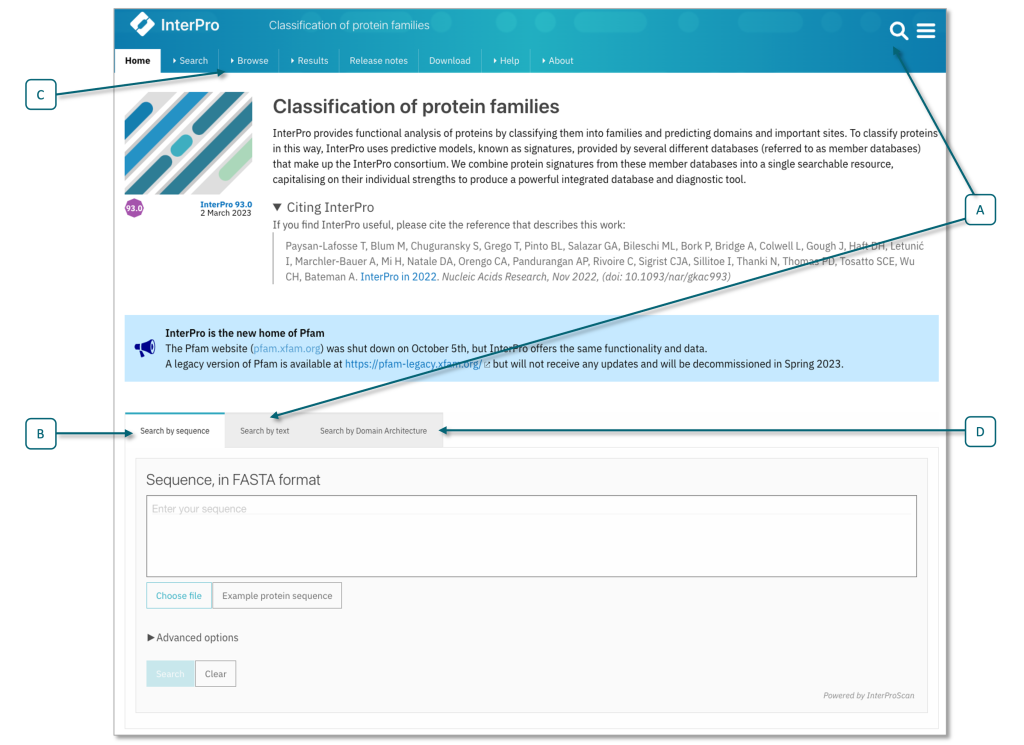
\includegraphics[width=1\linewidth]{files/interpro-search-6c154991474b34bbe8ce014cfbd76ce3.png}
\caption[]{Search fields on the InterPro home page, showing text search field (A) and the sequence search (B) options, including `Advanced options', where you can limit your search to member databases or sequence features of interest.
Selecting the browse tab in the top menu (C) allows access to a browse search, (e.g., search for member database signature, InterPro entry type), see also Figure~\ref{interpro-browse}.
You can also search for a particular domain architecture (D).
Credits: \cite{interpro_2022}.}
\label{interpro-search}
\end{figure}

\begin{figure}[!htbp]
\centering
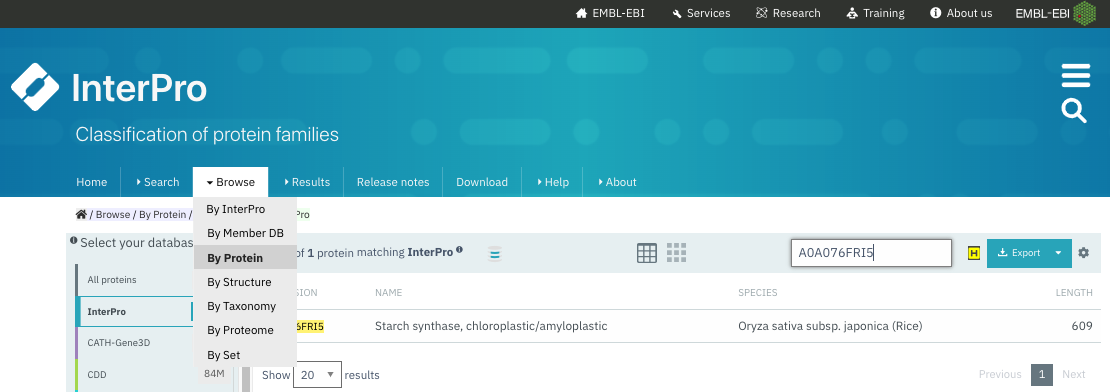
\includegraphics[width=1\linewidth]{files/interpro-browse-1ae9c2adc4608445ebe1acc3eca4156e.png}
\caption[]{Browse the annotated proteins in Interpro and search for a UniProt accession.
See resulting entry in (Figure~\ref{interpro-prot}). Credits: \cite{interpro_2022}.}
\label{interpro-browse}
\end{figure}

\begin{figure}[!htbp]
\centering
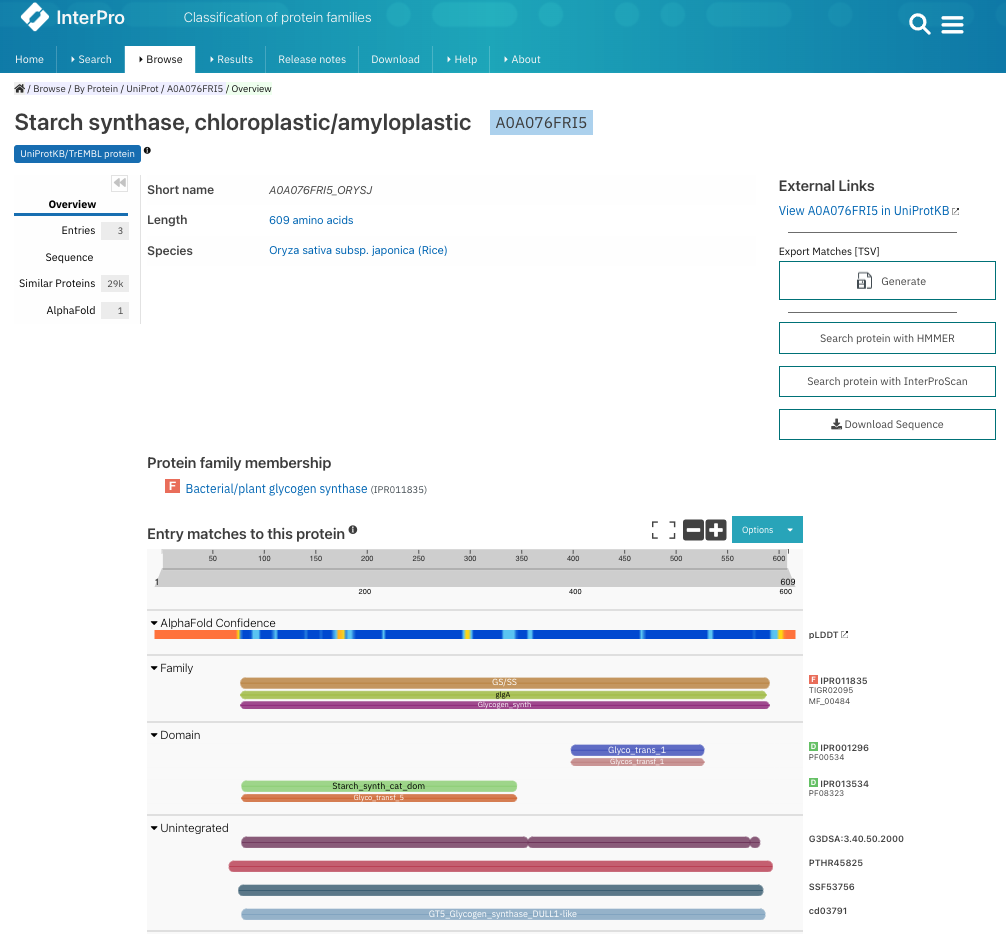
\includegraphics[width=1\linewidth]{files/interpro-prot-21d5398cff123b16fdb878429744a14e.png}
\caption[]{The result page when looking up UniProt accession \href{https://www.ebi.ac.uk/interpro/protein/UniProt/A0A076FRI5/}{A0A076FRI5} in InterPro.
You can see the family and domain annotation and on the right the accessions in InterPro and in the member databases.
You can click on each of these accessions to get to the entry information. Credits: \cite{interpro_2022}.}
\label{interpro-prot}
\end{figure}

You may have noticed a colored letter before each InterPro accession, e.g., F before IPR011835 or D before IPR001296 (Figure~\ref{interpro-prot}).
These icons denote the different InterPro entry types:

\begin{itemize}
\item (Homologous) Superfamily - a large diverse family, usually with shared protein structure.
\item Family - a group of proteins sharing a common evolutionary origin, reflected by their related functions and similarities in sequence or structure.
\item Domain - a distinct functional or structural unit in a protein, usually responsible for a particular function or interaction.
\item Repeat - typically a short amino acid sequence that is repeated within a protein.
\item Site - a group of amino acids with certain characteristics that may be important for protein function, e.g., active sites or binding sites
\end{itemize}

\begin{figure}[!htbp]
\centering

\includegraphics[width=0.4\linewidth]{files/interpro-types-5f7c10e9e25c86c696214d3eeac1e545.png}
\caption[]{The icons for the different InterPro entries (homologous superfamily, family, domain, repeat or site).
Credits: \href{https://creativecommons.org/licenses/by-sa/4.0/}{CC BY-SA 4.0} \cite{interpro-types_2020}.}
\label{interpro-types}
\end{figure}

\begin{framed}
\textbf{See Also}\\
You can find more information on InterPro entry types with examples \href{https://www.ebi.ac.uk/training/online/courses/interpro-functional-and-structural-analysis/what-is-an-interpro-entry/interpro-entry-types/}{here}.
\end{framed}

\paragraph{Pfam}\label{chapter1_pfam}

Pfam is an important resource for protein domains.
In Pfam, domains are classified according to profiles that are modelled as Hidden Markov models (HMMs).
We will learn more on HMMs in \href{/chapter2}{chapter 2}.

% #% Create a direct cross-link to HMMs in chapter 2 when written.

Pfam is now integrated in InterPro.
Each Pfam domain can be represented with a logo, where the amino acids frequent at a particular position are represented as larger letters (Figure~\ref{pfam-profile}).

\begin{figure}[!htbp]
\centering
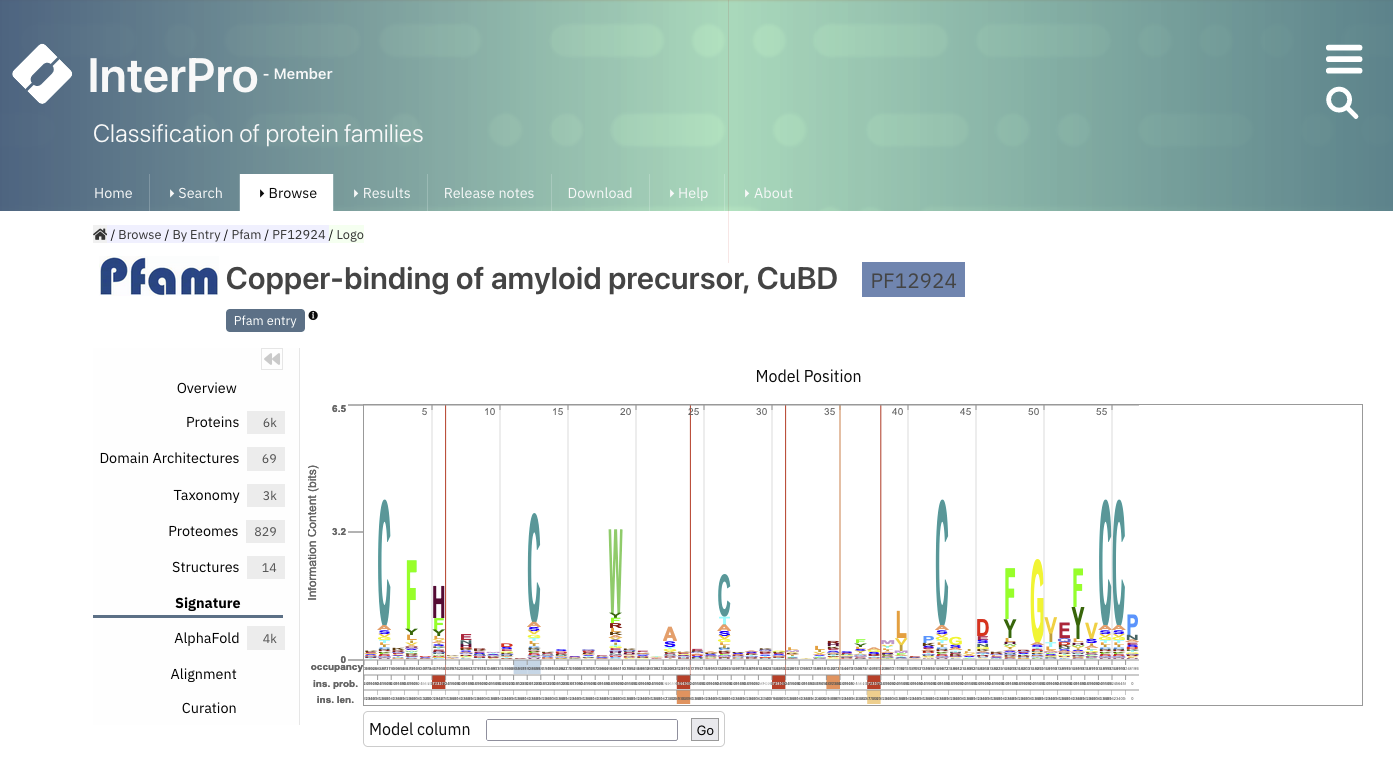
\includegraphics[width=0.7\linewidth]{files/pfam-profile-46bb7a5320328b531204cc524a214845.png}
\caption[]{The Pfam logo for PF12924.
Credits: \cite{interpro_2022}.}
\label{pfam-profile}
\end{figure}


\bigskip
\centerline{\rule{13cm}{0.4pt}}
\bigskip

\paragraph{File formats}

There are many different formats for biological data.
A format is a set of rules about the contents and organization of the data.
You should be familiar with a couple of common data formats in bioinformatics, which you will experience in the practicals.

\begin{framed}
\textbf{Note 1.8: Examples of common data formats in bioinformatics}\\
\begin{itemize}
\item FASTA
\item Genbank
\item GFF (Generic Feature Format)
\item FASTQ
\item SAM/BAM (Sequence Alignment/Map format)
\item VCF (Variant Call Format)
\item PDB (structure data)
\end{itemize}
\end{framed}

\subparagraph{Plain text files}

Many of the biological data formats are plain text files, they only contain letters, numbers, and symbols, but no formatting, such as font size or colors.
As a convention, they usually have the ending \texttt{.txt}.
The advantage of plain text files is that they can be opened with any text editor on any computer.
Plain text differs from rich text format, where the latter can also include formatting.
Many bioinformatics programs expect plain text files as input.
Thus, when creating them on your computer, take care to save in this format, and not for example in rtf or word.

On a Windows computer, plain text files can for example be created with the Notepad program (Figure~\ref{notepad}).

\begin{figure}[!htbp]
\centering
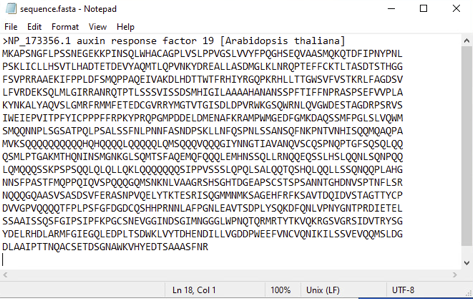
\includegraphics[width=0.7\linewidth]{files/notepad-5b8ceca90dcca4116236b117fb2fa376.png}
\caption[]{A screenshot of Notepad on Windows.
Credits: \href{https://creativecommons.org/licenses/by-nc/4.0/}{CC BY-NC 4.0} \cite{own_1_2024}.}
\label{notepad}
\end{figure}

On a Mac, plain text files can for example be created with the TextEdit program (Figure~\ref{textedit}).
Take care to set the settings to plain text.

\begin{figure}[!htbp]
\centering
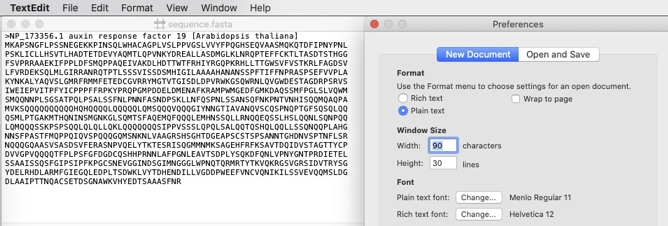
\includegraphics[width=1\linewidth]{files/textedit-0cc959f5c3e7cca8c6a83748cdd24856.png}
\caption[]{A screenshot of TextEdit on Mac.
Credits: \href{https://creativecommons.org/licenses/by-nc/4.0/}{CC BY-NC 4.0} \cite{own_1_2024}.}
\label{textedit}
\end{figure}

\begin{framed}
\textbf{See also}\\
If you are not yet familiar with plain text editors, then try it now and write and save a plain text file on your computer!
\end{framed}

There are some important file formats in bioinformatics.
A \textbf{fasta file} stores a DNA or protein sequence (Figure~\ref{fasta}).
Information on the sequence is found in the header (starting with \texttt{\textgreater }), which is on one line and the sequence can go over multiple lines.
A multi-fasta file stores multiple sequences.

\begin{figure}[!htbp]
\centering
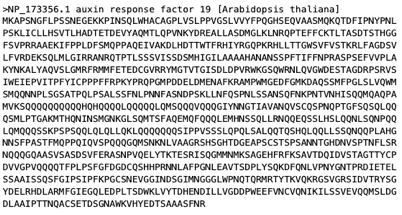
\includegraphics[width=0.5\linewidth]{files/fasta-838a5085fa938c75bc15fa75c6541b53.png}
\caption[]{A sequence in fasta format.
Credits: \href{https://creativecommons.org/licenses/by-nc/4.0/}{CC BY-NC 4.0} \cite{own_1_2024}.}
\label{fasta}
\end{figure}

The \textbf{GenBank file format} is a popular format to represent genes or genomes.
\href{https://www.ncbi.nlm.nih.gov/Sitemap/samplerecord.html}{Here} you can find an example GenBank record with annotations.
Important elements are the Locus, Definition (i.e., the name), and the Organism.
Additionally, Features, such as genes and CDSs (coding sequences) are listed.

\subparagraph{Binary files}

Binary files are all the files that are not text files, they cannot be opened in a text editor.
Instead, they need special programs to write and to open and interpret them.
Examples are word files (\texttt{.docx}) which can be opened with Word, pdf files (\texttt{.pdf}) which can be opened with Acrobat Reader, or image files (e.g., \texttt{.png}) which can be opened with image viewers.

Binary files are are also sometimes used in bioinformatics.
Examples include the bam format, which is a binary version of the sam format or the gzip format.
Gzip is used for compressing text files without the loss of information.
For large files, lots of disk space can be saved this way.


\bigskip
\centerline{\rule{13cm}{0.4pt}}
\bigskip

\subsubsection{Ontologies}\label{chapter1_ontologies}

An ontology is a comprehensive and structured vocabulary for a particular domain, such as biology, genetics, or medicine.
It defines the various terms used in a domain, along with their meanings and interconnections.
As such, ontologies serve as standardized frameworks for organizing and categorizing information in a way that enables effective communication and reasoning among researchers, practitioners, and computer systems.
For example, the terms in an ontology can encompass biological entities like genes, proteins, and cells, as well as processes, functions, and interactions that occur within living organisms.
Most of the databases mentioned mentioned in this chapter use ontologies in some way to describe their data.

Ontologies play a crucial role in bioinformatics because they facilitate:

\begin{enumerate}
\item \textbf{Standardization and consistency}: ontologies provide a common language and consistent framework for researchers and professionals, ensuring that everyone understands and uses terms in the same way.
\item \textbf{Interoperability}: ontologies facilitate the sharing and integration of data and knowledge across different research groups, institutions, and databases.
They enable computer systems to process data more accurately, leading to more meaningful analyses and discoveries.
\item \textbf{Scientific reasoning}: by organizing information in a logical and structured way, ontologies help researchers generate hypotheses, design experiments, and validate findings more effectively.
\end{enumerate}

\begin{framed}
\textbf{Note 1.9: FAIR principles}\\
As described above, ontologies facilitate scientific reproducibility.
A key concept in scientific reproducibility are the FAIR principles, with FAIR standing for Findable, Accessible, Interoperable, and Reusable.
This reader does not describe them in detail, but you should read the following online resource to familiarize yourself with the \href{https://www.go-fair.org/fair-principles/}{FAIR principles}.
\end{framed}

Ontologies typically form a hierarchy, where specific terms point to more generic terms. More generally, most ontologies are represented as a graph, where ontology terms are the nodes and relationships between terms are edges. As such, one ontology term may have more than one parent term.

A variety of ontologies are frequently used in the life sciences, some of which are discussed in greater detail below.

\paragraph{Gene Ontology}\label{chapter1_gene_ontology}

The \href{http://geneontology.org/}{Gene Ontology} (GO) is a knowledgebase for the function of genes and gene products (e.g. proteins). It is organised into three different domains covering various aspects:

\begin{itemize}
\item Molecular Function: molecular-level functions performed by gene products (e.g. proteins), such as `catalysis' or `transport'.
Most molecular functions can be performed by individual gene products, but some functions are performed by complexes consisting of multiple (possibly differing) gene products.
GO molecular functions often include the word ``activity'' (an \textit{amylase} enzyme would have the GO molecular function \textit{amylase activity}).
\item Cellular Component: the cellular structures (or location relative to them) in which a gene product performs its function.
Can be cellular compartments (e.g., \href{http://amigo.geneontology.org/amigo/term/GO:0005739}{mitochondrion}) or macromolecular complexes of which they are part (e.g., the \href{http://amigo.geneontology.org/amigo/term/GO:0005840}{ribosome}).
\item Biological Process: the larger biological programs composed of multiple molecular activities, for example \href{http://amigo.geneontology.org/amigo/term/GO:0006281}{DNA repair} or \href{http://amigo.geneontology.org/amigo/term/GO:0007165}{signal transduction}.
\end{itemize}

\begin{framed}
\textbf{Note 1.10: Molecular pathway?}\\
A biological process is not equivalent to a molecular pathway.
At present, the gene ontology does not represent the dynamics or dependencies that would be required to fully describe a pathway.
\end{framed}

A good example of how ontologies are represented as graphs is the biological process \href{http://amigo.geneontology.org/amigo/term/GO:0019319}{hexose biosynthetic process}, which has two parents: \href{http://amigo.geneontology.org/amigo/term/GO:0019318}{hexose metabolic process} and \href{http://amigo.geneontology.org/amigo/term/GO:0046364}{monosaccharide biosynthetic process}.
This reflects that biosynthetic process is a subtype of metabolic process and a hexose is a subtype of monosaccharide. (Figure~\ref{go}).

Edges between GO terms in the GO hierarchy can represent various relationships between genes and gene products.
The four main relationship types used in the gene ontology are `is a', `part of', `has part', and `regulates' (see Figure~\ref{so}).

\begin{figure}[!htbp]
\centering
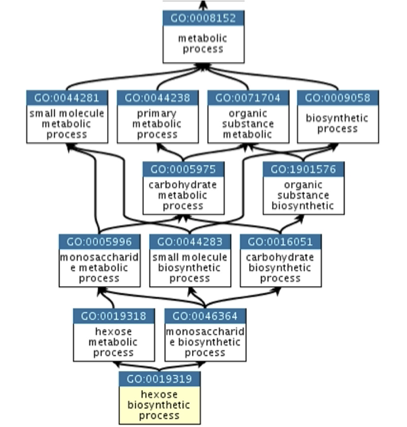
\includegraphics[width=0.55\linewidth]{files/go-67ecfd572d47f6ed3bdc35c0013264b8.png}
\caption[]{An extract of the Gene Ontology hierarchy.
Credits: \cite{go_2009}}
\label{go}
\end{figure}

\paragraph{Sequence Ontology}\label{chapter1_sequence_ontology}

The \href{http://sequenceontology.org}{Sequence Ontology} (SO) describes biological sequence elements such as genes or repeats, along with their features and attributes.

The sequence ontology is organized on four main levels:

\begin{itemize}
\item Attribute: an attribute describes a certain quality of a given sequence, for example the sequence source (i.e., how it was generated).
\item Collection: multiple discontiguous sequences together, for example the chromosomes of a complete genome.
\item Feature: the most general top-level entry that describes any extent of a continuous biological sequence, for example a \href{http://sequenceontology.org/browser/current\_release/term/SO:0000704}{gene} is a \href{http://sequenceontology.org/browser/current\_release/term/SO:0000001}{region}, which in turn is a sequence feature.
\item Variant: intended to describe genetic variation. The definition of a sequence variant is composed of other entries in the sequence ontology: ``A \href{http://sequenceontology.org/browser/current\_release/term/SO:0001060}{sequence\_variant} is a non-exact copy of a \href{http://sequenceontology.org/browser/current\_release/term/SO:0000110}{sequence\_feature} or \href{http://sequenceontology.org/browser/current\_release/term/SO:0001026}{genome} exhibiting one or more \href{http://sequenceontology.org/browser/current\_release/term/SO:0001059}{sequence\_alterations}''
\end{itemize}

\begin{figure}[!htbp]
\centering
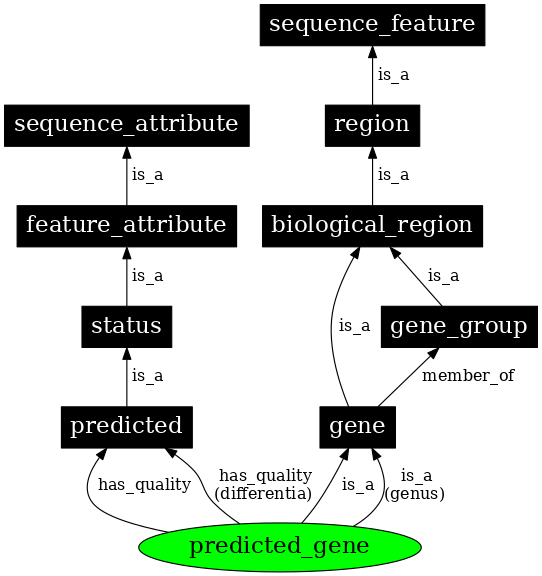
\includegraphics[width=0.4\linewidth]{files/sequence_ontology-3ebb78a944729d0afd7391447a463a9f.png}
\caption[]{An extract of the Sequence Ontology hierarchy.
Credits: \cite{so_2005}.}
\label{so}
\end{figure}

\paragraph{Other ontologies}\label{chapter1_other_ontologies}

Many more ontologies exist and are relevant to biomedical research.
The European Bioinformatics Institure (EBI) provides an \href{https://www.ebi.ac.uk/ols4/}{ontology lookup service} that facilitates searching for ontologies.
Examples of other ontologies are the \href{https://www.ebi.ac.uk/ols/ontologies/po}{plant ontology} that describes various anatomical structures in plants, and the \href{https://disease-ontology.org/}{human disease ontology}.


\bigskip
\centerline{\rule{13cm}{0.4pt}}
\bigskip

\subsubsection{Practical assignments}

This practical contains questions and exercises to help you process the study materials of Chapter 1.
You have 2 mornings to work your way through the exercises.
In a single session you should aim to get about halfway through this guide (i.e., day 1: assignment 1-3, day 2: assignment 4 and project preparation exercise).
Use the time indication to make sure that you do not get stuck in one assignment.
These practical exercises offer you the best preparation for the project.
Especially the \textbf{project preparation exercise} at the end is a good reflection of the level that is required to write a good project report.
Make sure that you develop your practical skills now, in order to apply them during the project.

\textbf{Note, the answers will be made available after the practical!}

\begin{framed}
\textbf{\textbf{Project Preparation Exercise}}\\
We want to obtain insights into members of the ARF gene family in \textit{Arabidopsis thaliana}.
ARF5 (UniProt ID P93024) and IAA5 (UniProt ID P33078) are two well-studied \textit{A. thaliana} proteins that play a role in auxin-mediated regulation of gene expression.
They are therefore chosen here as the starting points for exploring the plant ARF gene family.
Perform a small background study on ARF5 and IAA5.
Explore the protein sequences, properties (e.g., length, composition, etc.), interaction partners, and functional regions of ARF5 and IAA5.
Finally, explore the genes encoding ARF5 and IAA5 in \textit{A. thaliana} (genomic location, exon structure, expression, etc.).

Describe the following items in a few bullet points each.
You may include up to two figures or tables.

\begin{enumerate}
\item \textbf{Materials \& Methods} What did you do? Which data, databases and tools did you use, and why did you choose these? What important settings did you select?
\item \textbf{Results} What did you find, what are the main results? Report the relevant data, numbers, tables/figures, and clearly describe your observations.
\item \textbf{Discussion \& Conclusion} Do the results make sense? Are they according to your expectation or do you see something surprising? What do the results mean, how can you interpret them? Do different tools agree or not? What can you conclude? Make sure to describe the expectations and assumptions underlying your interpretation.
\end{enumerate}
\end{framed}

\subsubsection{Glossary}